\documentclass[output=paper]{LSP/langsci} 
\ChapterDOI{10.5281/zenodo.1441341}
\author{Timo Buchholz\affiliation{Freie Universität Berlin}\lastand Uli Reich\affiliation{Freie Universität Berlin}}
\title{The realizational coefficient: Devising a method for empirically determining prominent positions in Conchucos Quechua}
\shorttitlerunninghead{Determining prominent positions in Conchucos Quechua} 
 
\abstract{We initially sketch a phonological theory in which the culminativity of word accents acts as only one out of four main functional goals for the configuration of prosodic devices and claim that languages exhibit many differences therein. Thus, in the study of many languages whose prosody is not extensively studied, as is the case for most languages spoken in situations of plurilingualism together with Romance Languages, we need reliable methodologies to determine their particular organization of time, tone, segmental strength and intensity. Using data from a Central Quechua dialect, we propose such a method consisting of a complex pragmatic and metrical annotation in {Praat} and its statistical exploration in R. We conclude with a discussion of preliminary results and shortcomings to be resolved.}

% {Keywords: Acoustic correlates of stress, Conchucos Quechua, Cumulative stress, Phonological distinctiveness, Semi-spontaneous data, Culminativity} 

\maketitle
\begin{document}
\label{chap:buc}\label{ch:4}

\section{The phonological perspective: Competing motivations of prosodic devices}
In the study of the phenomena involved in what has been called ``\isi{accent}'', ``stress'' and\slash or ``\isi{prominence}'' in different and partially incompatible terminologies,\footnote{See \citet{Beckman1986} for an impressively well-informed historical overview that sheds some light on the genesis of the terminological confusion and suggests ways out of it. Note that her own typological proposal is privative: non-stress languages are languages that are defective with regard to the set of properties that define stress languages. In the following, we will use the term \textsc{word accent} to designate the abstract phonological knowledge of one and only one \isi{syllable} in a \isi{prosodic word} that is perceived as stronger than all other syllables in that word. In principle, it does imply neither the \isi{phonetic} cues that may realize it in a given stretch of speech, nor the phonological domain that projects it. Accents can be specified in the lexicon or projected by metrical algorithms that construct alternating \textit{prominence} in a hierarchically ordered metrical grid. In the latter case, word accents are the topmost prominent position in such a grid. The term ``stress'', as it is used in the literature, is widely synonymous with our notion of ``\isi{word accent}'', but implies also aspects of its realization, as in the typological dichotomy of {stress-accent} and {pitch-accent} languages. Since we want to keep these notions strictly apart in order to describe their relation precisely, we will avoid the term ``stress'' wherever it is possible, in spite of its widespread usage in the literature we rely on.} we can draw a line of progress in typological research that puts the universality of the assumption that every \isi{phonological word} has a single primary \isi{accent} into question. Early structuralist theory \citep{Trubeckoj1939} used ``main tone'' (germ. \textit{Hauptton}) to illustrate the \textit{culminative} (germ. \textit{gipfelbildend}) function in phonological systems as opposed to the \textit{delimitative} and the \textit{distinctive} functions. An \isi{accent} was conceived of as being ``\is{accent!culminative}culminative'' in the sense that it is the most prominent position in a syntagmatic sequence of hierarchically organized accents. Later, \is{accent!culminative}culminativity was developed as a core concept of Metrical Phonology in order to derive ``stress'' by the hierarchical build-up of \isi{prominence} in metrical grids (\citealt{Liberman1977}: 262; \citealt{Hayes1995}: 24–25). 

In many languages, sometimes called ``stress-\isi{accent} languages'', accents are also ``accumulative'' in the sense that they attract all out of four possible \isi{prosodic} parameters, namely intensity, duration, pitch and segmental strength. Thus, an accented \isi{syllable} is believed to show salient pitch events, to be longer, to not reduce vowels, or even diphthongize them (traditionally, the preference for accented syllables for being bimoraic has been coined in Prokosch’s Law), to show more complex onsets and codas and to be louder. 

A glance at the phonological configuration of tone languages, however, shows that a conception of word accents that accumulate all \isi{phonetic} instances of \linebreak strength does not hold cross-linguistically. In tone languages, tones can be associated with many syllables in one word, as \citet{Yip2002} shows in her seminal work. See her example from \ili{Chilungu}, a language from the \ili{Bantu} family, in which one tone is associated with many vowels \citep[68]{Yip2002}:


\ea
% [Warning: Draw object ignored][Warning: Draw object ignored][Warning: Draw object ignored][Warning: Draw object ignored][Warning: Draw object ignored]
%\todo[inline]{redraw links}
\label{ex:buc:1}  
\glll kú-sóóbólól-à   k\tikzmark{ku}u-s\tikzmark{so}o\tikzmark{o1}ob\tikzmark{o2}ol\tikzmark{o3}ol-a\\
      ~				~ \\
     to~sort~out     H\tikzmark{H}  \\
     
\z
\connect{H}{ku}\connect{H}{so}\connect{H}{o1}\connect{H}{o2}\connect{H}{o3}

As \citet{Yip2002}, among many other scholars working on tone languages, shows convincingly, this one-to-many relation is not the end of the story; many languages also show the inverted relation, associating many tones with the nucleus of one \isi{syllable}, a situation that is familiar from boundary tones found in many intonational languages.

Duration can also show up without strict association with a \isi{word accent}. Thus, in \ili{Wolof}, a Western Atlantic language spoken in Senegal without distinctive tones at the word level, both vowels and consonants show distinctive duration, both for lexical contrasts (\ref{ex:buc:2}a, b) and the expression of focus (\ref{ex:buc:2}c, d).\footnote{Note that the contrasts in (\ref{ex:buc:2}c) and (\ref{ex:buc:2}d) appear as focus morphology in the literature. In other cases of the focus system, the morphological contrasts are expressed by segmental modification and addition. See \citet{Voisin-Nouguier2002} and \citet{Rialland2001} for the full system.} Long syllables (bimoraic, hence heavy) are possible in basically every position \REF{ex:buc:3} and in more than one position in the word \REF{ex:buc:4} (examples from \citealt{Ka1989,Ka1994} and \citealt{Voisin-Nouguier2002}).

\ea
    \label{ex:buc:2}
  \ea
  \gll fat~~~ :~~~ faat  \\
    clean.up ~ kill \\  
  \ex
    gën~~~ :~~~~ gënn\\
    better ~~~~ milk\\
  \ex
  \gll ma dem~~~ :~~~ maa dem                   \\
	I go ~ [I]\textsubscript{Foc} go    \\
  \ex
  \gll mu dem~~~  :~~~ moo dem\\
      he goes  ~  [he]\textsubscript{Foc} goes\\
     
  \z
\z


\ea%3
    \label{ex:buc:3}
  \ea
  \gll \textipa{"}boole\\
  mix\\
  \ex
  \gll te\textipa{"}raanga \\
  hospitality\\
  \ex
  \gll \textipa{"}dajaloò\\
  gather\\
  \z
\z

\ea%4
    \label{ex:buc:4}
    \ea
    \gll\textipa{"}woowandòo  \\
    call.together  \\
    \ex 
    \gll \textipa{"}feesalukàay   \\
    instrument.used.to.fill\\
    \ex
    \gll ji\textipa{"}géénubìir \\
   pregnant.woman \\
\z
\z

\ea%5
    \label{ex:buc:5}
    \ea
    \gll \textipa{"}tabax \\
	build \\
    \ex
    \gll \textipa{"}ndaje\\
    meeting  \\
    \z 
\z 

\citet{Ka1989,Ka1994} claims that in instances of words with light syllables only and in words with one or more heavy (=long) \isi{syllable}, the first (\ref{ex:buc:3}c, \ref{ex:buc:5}) or the first heavy \isi{syllable} (\ref{ex:buc:3}b, \ref{ex:buc:4}c), respectively, receives stress. If the heavy \isi{syllable} occurs after two light ones (\ref{ex:buc:3}c), it is perceived as having secondary \isi{prominence}, while primary \isi{prominence} falls on the \isi{initial syllable}. In this language, then, duration appears as being as independent from a \is{accent!culminative}culminative word accent as tone is in so-called tone languages. As we shall see, the Central \ili{Quechua} dialects show a distribution of length that comes close to this phonological constellation. \ili{Finnish} and Latin are European Languages that show distinctive duration independent from \isi{word accent}, but Latin shows some restrictions that \ili{Finnish} does not have. \ili{German} is a quantity language that comes quite close to a ``prototypical stress \isi{accent} language'': it has vocalic duration only in ``stressed'' syllables \citep{Becker1996}. Thus, the independence of duration from \isi{word accent} shows varying degrees and it is far from clear where we should set the threshold to tell types apart.


Another feature of word accents is that the nuclei of the syllables that bear it, unlike its neighbors, are never reduced, rather often diphthongized and that they show more segmental contrasts than the nuclei of other syllables. Interestingly, exactly this feature has been shown repeatedly as being dependent on what has been called the rhythm type of a given language (\citealt{Dauer1983,Auer1993,Auer2001,Dufter2003}). In \ili{Romance} languages, e.g., it holds for European \ili{Portuguese}, which shows exactly the vocalic reductions and consequently strong restrictions on segmental inventory claimed as general properties of syllables less prominent than the one with the \isi{word accent} in word rhythmic languages (formerly ``stress-timing''). It does not hold as clearly for most varieties of \ili{Spanish}, Standard \ili{Italian} or even \ili{Brazilian Portuguese}, that are taken as instances of \isi{syllable} rhythmic languages (formerly ``syllable-timing'', \citealt{Abaurre1998,Reich.2002}), but in \ili{Brazilian Portuguese}, vocalic reduction still occurs more than in \ili{Spanish} and \ili{Italian}. 

In \ili{Spanish}, the only property of lexical phonology related to the preference of word accents to be bimoraic is the distribution of diphthongs (cf. \textit{/beneˈswela/} vs. \textit{/benesoˈlano/}), while the nuclei of all syllables are fully pronounced in most cases. However, there can be no doubt at all that \ili{Spanish} does have a \isi{word accent} that invariably is the locus of major tonal events if they are realized. It is simply less dominant than its European \ili{Portuguese} counterpart is. Again, we find different constellations of features that are held to define types. Where should we draw the line?

The last feature we want to mention in this complicated introduction is intensity. Intensity does not seem to play any phonological role at all but as a feature of word accents. \citet[160]{Beckman1986}, however, it shows that this property cannot be generalized across languages, since in \ili{Japanese} intensity is independent from the position of the accented \isi{syllable}. Intensity, then, also fails to form a universal feature of the strongest \isi{syllable} in the word. 

Given these facts, \is{accent!culminative}culminativity rather seems to describe an optional than a universal concept of accents. We hypothesize that \is{accent!culminative}culminativity is a functional principle that is counterbalanced by others. Distinctivity is directly antagonistic, as it dissociates time, tone, segmental quality and intensity to enhance the possibilities of paradigmatic contrast for \isi{phonological word} forms. Thus, the \is{accent!culminative}culminativity of word accents grows at the expense of the distinctive potential of \isi{prosodic} devices. Vice versa, the use of \isi{prosodic} devices for distinctive functions levels the dominance of word accents, since time, tone, sonority and intensity can be distributed over different positions in the word or phrase. Delimitation may conspire with \is{accent!culminative}culminativity towards the overall target of identifying words or phrases in a given chain of speech, but in all systems with non-peripheral \isi{word accent}, boundary tones, final lengthening and segmental processes like consonantal strengthening and epenthesis of glottal stops are also likely to diminish the \isi{phonetic} saliency of the \isi{syllable} bearing \isi{word accent}. Another core function of accents, absent in structuralist phonology, is rhythmicity, as recognized since the early days of Metrical Phonology (\citealt{Liberman1977,Hayes1995}), but put into a theoretical framework that takes \is{accent!culminative}culminativity as universal and thus misses the functional particularities between different aspects of \isi{prosodic} form. In many languages, the assignment of primary accents does not depend on foot construction (\citealt{Hulst1999}: 72). Rather, the assignment of alternating strengths of acoustic events in time appears to be an independent functional domain of \isi{prosody} with which lexical accents may, but need not, coincide. The functional target of rhythmicity surely is neither distinctivity, nor \is{accent!culminative}culminativity, nor delimitation. To the contrary, it enhances the isochronous distribution of alternating \isi{prominence} at the expense of all the three functions recognized by the Prague school.

In our view, particular phonologies are organized as instances of decisions between (at least) these major functional goals. Ideal types can be set as abstract possibilities that no language ever reaches because of the competing drives towards the other ends of this space of \isi{prosodic} possibilities. In the ideal type of a \is{accent!culminative}culminative \isi{prosodic} system, tonal events, duration, segmental strength and intensity would occur but in the one and only prominent \isi{syllable} of every word. In the ideal type of a distinctive \isi{prosodic} system, tones, duration, segmental contrasts and intensity are scattered all over and boundaries between words or phrases are blurred. In the ideal type of a delimitative \isi{prosodic} system, tones, duration and intensity occur at the boundaries of wordless phrasal chains without \isi{prominence}. Finally, in the ideal type of a rhythmic \isi{prosodic} system, we would find isochronally recurring contours of \isi{prominence}, just as in music (\citealt{Reich2014}). Natural phonologies balance the competing drives towards these ideal types as they fulfil their communicative goals in the variational space of human languages, constrained by universal cognitive principles and the historical traditions of social networks. 

In the end, the view we are defending aims at the abolition of dichotomic typologies and pleads for their passage to particular phonological configurations within a polydimensional space defined by competing functional principles. This is very much in line with, while a step more radical than, views on \isi{prosodic} typologies defended by \citet{Hyman2009,Hyman2014}, in his impressive command of facts from the phonologies of many languages in the world.\footnote{The main difference is probably that Hyman still recognizes the typological validity of concepts such as ``stress \isi{accent} language'' and ``tone language'', while the relevant configurations are only possibilities among others in our \isi{prosodic} universe.} He comes to a conclusion that is not only wise for theory building, but also mandatory for the great empirical endeavor of the study of language: it is better to look at what languages do than to brood upon fictitious universals. 

Research into the \isi{prosodic} phonologies of languages that are not very well known, as is the case for most contact languages of the \ili{Romance} languages outside Europe, must bear in mind that any constellation of the main \isi{prosodic} devices may be the case in the language under study. Thus, they must be controlled for independently, but in relation to each other. And we can take nothing for granted. 

\section{The project and a short overview over the method of data elicitation}

The methodological considerations we will expose in the following pages are part of our research project \textit{Zweisprachige Prosodie: Metrik, Rhythmus und Intonation zwischen Spanisch und Quechua} (`Bilingual \isi{prosody}: metrics, rhythm and \isi{intonation} between \ili{Spanish} and \ili{Quechua}'), funded by the Deutsche Forschungsgemeinschaft. The overall goal of the project is the development of a \isi{prosodic} theory of bilingualism on empirical grounds.

Our data was gathered through fieldwork in Huari, Conchucos, Ancash, Peru during the months of September-October 2015. The elicitation methodology aims at producing semi-spontaneous data, that is, speech produced naturally in dialogues under pragmatic and lexical constraints, in turn influencing \isi{prosody}. Informants were asked (always in pairs) to play the following dialogical games in which any interaction could only be done orally, gestures were not permitted:

\begin{enumerate}
\item {Picture-naming}. Participants had to name objects shown to them on picture cards.

\item {A version of memory}. Participants took turns guessing where a certain picture on a card was. The cards had been shown to them for a short time and then flipped over. 

\item {Map-task} \citep{Anderson1991}. Participants were provided with two maps, one with a path drawn between the objects shown on it, the other without the path. They were not allowed to see each other’s maps. The participant with the map had to explain the path to the other one, who had to follow it by drawing it on their own map. The maps differed in some of the objects shown. Resulting communicative conflicts had to be resolved orally.  

\item {Story re-telling}. Participant A would listen to a recording of a story (invented by the investigators and spoken for the recording by their local collaborator and advisor, \ili{Quechua} teacher and native speaker Gabriel Barreta (GB)\footnote{Our deep gratitude and friendship goes to Gabriel Barreta and his family in Huari as well as to Leonel Menacho López and his wife Ana in Huaraz, who have provided invaluable help with local logistic and linguistic questions and without whom our fieldwork could not have been successful.} ). They would then tell the story to the other participant B, who had been waiting outside while the recording was playing. After being told the story, participant B would tell the story to one of the interviewers, with the possibility of correction by participant A. 

\item {A version of “Who am I?”}. Participant A would be told the name of a person known to both participants, and participant B had to guess the person’s identity.

\item {Guessing the contents of boxes}. Both participants were provided with closed cardboard boxes and would take turns guessing their contents from just moving the boxes, shaking or weighing them by hand. 
\end{enumerate}


The content items of games 1--4 were restricted by means of the props provided, i.e. the cards, the maps and the recordings, to consist mostly of a set of lexical items varying through the possibilities of \ili{Quechua} syllabic and moraic structure. Hence, the pictures on the cards displayed objects aimed at eliciting words ranging from two light (L) syllables to two heavy (H) and one light \isi{syllable}, e.g. \textit{tsu.ku} (L-L) `hut', or \textit{qi.llay.yuq} (L-H-H) `rich man'. The subsequent games utilized the same lexical items (elicited by means of the same pictures, also on the maps, or the recording) wherever possible. Adjustments to these items were made after a first trial session with our principal local collaborator GB, who gave us local words for several of the metrical constellations that were to be elicited. 

Care was taken to have the experiments take place in rooms that were as quiet as local conditions allowed. Participants would play the games in both \ili{Quechua} and \ili{Spanish}, going through all the games first in one language, and then the other. Audio recordings of the games were made using a Marantz PMD 670 audio recorder in connection with a Røde NT-1A condenser microphone in 44.1\,KHz PCM. In total, excluding the trial with GB, 40 participants (22 females, 18 males, all bilinguals, mean age=22 years) were recorded in 20 sessions, yielding about 7 hours of \ili{Spanish} and 6 hours of \ili{Quechua} experimental data. All informants participated voluntarily, gave us their written consent to be recorded and for the resulting data to be published maintaining their anonymity, and were remunerated for their participation.   

\section{Methodology}
\label{sec:buc:3}
\subsection{The challenge: determining prosodic constellations on empirical grounds}

As far as we know, the determination of positions of \isi{prominence} in a language where they are unknown has not been studied extensively. In grammatical treatments of understudied (i.e., almost all non-European) languages, \isi{accent} placement usually is dealt with cursorily: the author describes the positioning of strong\-est \isi{prominence}, sometimes differentiating between several acoustic realizations, in a seemingly intuitive manner. Matters such as \isi{accent} domain, acoustic correlates, function of \isi{prominence} and interaction with other \isi{prosodic} phenomena are rarely dealt with in systematically ordered empirical procedures, but attributed by intuition. Effectively, this means that the describing linguist “hears” \isi{accent} positions in the language of their informants and generalizes from this audio perception. While we recognize that this was the only methodology available in many cases, we submit that it is not a methodology appropriate for scientific research since it allows for a number of non-trivial descriptive distortions due to perceptual biases on behalf of the describing linguist.\footnote{To clarify: our goal is by no means to insult or belittle the efforts of linguists that have done extensive research on otherwise little studied languages. We applaud their endeavors and think that both we and the linguistic community in general are highly indebted to them. However, many of these studies took place several decades ago, when \isi{prosodic} theory was even more in its infancy than it is today and when, even more crucially, large-scale audio recordings of small languages that could be analyzed appropriately and shared with the academic community were not feasible, due to technical and logistic problems. Many of these researchers had to make do with what they had, and it is no doubt better that they gave an impressionistic description of \isi{accent} systems in their languages than none at all. Nonetheless we think it is time that with the technical means at our disposal, the methodology to describe \isi{prominence} systems in these languages should be reevaluated.}  If the linguist’s first language is one where the lexical \isi{accent} is \is{accent!culminative}culminative and accumulative, as for example in English or \ili{German}, then we cannot discard the possibility that this phonological background will influence them to a certain degree in their perception of the language they are studying. This will be even more the case if the linguist in question is not a specialized phonologist who might be aware of their own biases in this regard. With the concept of a universal \is{accent!culminative}culminative word accent, one is already excluding a large subset of the possible shapes \isi{accent} systems assume (see, e.g., \citealt{Hyman2014} for an overview, and \citealt{Kuegler2012} for a particularly diverging case). 

Moreover, in the case of the so-called central dialects of \ili{Quechua}, we are faced with distinctive length, whose interference with \isi{accent} placement and realization has never been discussed, and a considerable disagreement even in the existing (impressionistic) literature on \isi{accent} position, domain and its acoustic correlates. Some of these dialects are described as having primary \isi{accent} on the penult (\citealt{Trager1945} for Huaraz \ili{Quechua}, \citealt{Parker1976} for Ancash-Huaylas \ili{Quechua}, \citealt{Adelaar1977} for Tarma \ili{Quechua}), others (and sometimes the same by another author) as having it on the \isi{initial syllable} of the word (\citealt{Parker1976} for Huaraz \ili{Quechua}, \citealt{Hintz2000} for Corongo \ili{Quechua}, \citealt{Hintz2006} for South \il{Quechua!Conchucos}Conchucos Quechua). In most cases, a secondary \isi{accent} is said to exist on the ``other'' position, i.e. penult or \isi{initial syllable} (all of them agreeing at least that no other position is a strong contender), and that their \isi{prominence} ranking can be reversed under certain morphological, pragmatic or conversational conditions (none of which are agreed upon by any two authors); some recognize a kind of division of labor between acoustic correlates in the realization of prominent positions. Our own visual and acoustic inspection of our own data does nothing to let us decide tentatively in favor of any of the hypotheses suggested in the literature. In fact, it complicates matters, since we often encounter utterances almost entirely devoid of any phrase-internal intonational movement that could reasonably be correlated with lexical \isi{pitch accent} positions. Intonational movement, if it occurs, seems to respond to a domain above the word and to be severely restricted in its inventory: Utterance-initial rises and utterance- or possibly phrase-final falls and rises are almost exclusively observed. From this inspection, the hypothesis that our \ili{Quechua} variety does not assign an \isi{accent} position at the lexical level seems to be at least as probable as any of the suggestions cited above. Another problem is that speakers generally do not receive any education on \ili{Quechua} and a very traditional one on \ili{Spanish}, and a bias that accords \ili{Spanish} greater prestige in academic matters definitely persists. Hence, speaker perceptions on where an “\isi{accent}” might lie in a given \ili{Quechua} word and what it might consist of are, if they exist at all, heavily influenced by these social conditions. We therefore thought it necessary to devise a methodology that would help us determine positions of \isi{realizational strength} from the speech signal, in order to determine without such biases (inherent also in our own perceptions) the nature and domain of regular prominences in the Conchucos variety of \ili{Quechua} our data is from. In the present study, semi-spontaneous data is used. Hence, phenomena of \isi{speech style} and individual style are also included in the data. Further research could however easily apply the same method to more controlled data. In the remainder of the text, whenever we say something about “\ili{Quechua}” without further variational qualification, we mean it to be about the variety of \ili{Quechua} spoken in Huari, Conchucos, studied by us.  

\subsection{Goals of the present contribution}
While the goal of our overall research project is the development of a \isi{prosodic} theory of bilingualism on empirical grounds, the present contribution does not yet aim so high. Faced with the conflicting descriptions in the literature and our own data regarding \isi{accent} placement described above, we think it is important to devise a methodology which arrives at a less biased description of the acoustical data we base our phonological theories on. Given that the question of the domain of \isi{accent} placement is absolutely vital for any hypotheses regarding the behavior of \isi{prosodic} domains in a plurilingual context, we take this to be an inevitable first step. Hence, the goal of this contribution is not to say anything about \ili{Quechua}-\ili{Spanish} bilingualism, but to provide evidence for the feasibility and usefulness of its methodology in helping us derive hypotheses about \isi{accent} placement in a language where this is not known; more specifically, to investigate the possibility by means of acoustic measurements that our variety of \ili{Quechua} does not assign \isi{accent} at the lexical level.\footnote{There is a substantial body of literature on \ili{Spanish}-\ili{Quechua} bilingualism with regard to all levels of linguistic description, including \isi{prosody}, such as \citet{ORourke2005,ORourke2007,ORourke2008,ORourke2009,Muntendam2010,ORourke2010,ORourke2012,Muntendam2012a,Muntendam2012b,Rijswijk2014,Muntendam2016,Muysken2016}. All of it is concerned with Southern or Ecuadorian varieties of \ili{Quechua} (that are more closely related to each other than to Central Quechuan varieties), where \isi{accent} placement seems not to be problematic. Due to the fact that in other systematic domains of the language, such as morphology and segmental phonology, the Southern and Ecuadorian varieties are different enough from the Central ones as a whole (not considering their considerable internal variation) to be judged mutually unintelligible, we are hesitant to just assume that the findings in the literature on the interaction between Southern \ili{Quechua} and \ili{Spanish} \isi{intonation}, e.g., can easily be applied to our variety. Mountainous regions notoriously harbor enormous variation in a relatively small geographic area, that this applies also to the realm of \isi{prosody} is by now well-known at least from the case of the varieties of Basque, where more or less every \isi{prosodic} parameter regarding \isi{accent} placement can be found (cf. e.g. \citealt{Hualde2008basque}; \citealt{Hulst2010,Aurrekoetxea.2012}). That the varieties of \ili{Quechua} vary with regards to their \isi{accent} placement to a considerable degree has also been recognized, see \citet{Wetzels2010}. Our goal here is only to provide a better basis for a description of the \isi{accent} placement in the variety of \ili{Quechua} we are studying. Only in subsequent studies will we hopefully have to say something about bilingualism.}  While all analytical tools and statistic procedures are not new in particular, their complex application to metrical and pragmatic variables has not been endeavored in any empirical \isi{prosodic} project we know of.

\subsection{Methodology – annotation} 
All the usable \ili{Quechua} data elicited through the means of the communicative games outlined in section 2 were transcribed and translated by bilingual students of the Universidad Nacional Santiago Antunez de Mayolo (UNASAM) in Huaraz, Ancash, Peru, and morphologically glossed by students of the Pontificia Universidad Católica del Perú (PUCP) in Lima, Peru using {ELAN} \citep{Wittenburg2006}. All further annotations were done by one of the authors as diligently as possible. In a follow-up investigation on a larger corpus we will also have a part of the corpus annotated by two independent annotators in order to arrive at a measure of inter-annotator agreement. 

\subsubsection{Syllables} 
Using a corrected version of the transcription as basis, we built on it by adding a syllabic annotation on a map-task by two male speakers (FB03 and WB04) in {Praat} (\citealt{Boersma.praat}). An example of what the \isi{syllable} annotation looks like can be found in Figure \ref{fig:buc:1}. Tiers 4 and 5 in the {Praat} textgrid are reserved for \isi{syllable} annotation (one tier for each speaker). Annotation boundaries were aligned as closely as possible with corresponding beginnings and endings of segmental material. A transcription system was used that aims at grouping together segments belonging to the same relevant class in \ili{Quechua}. 

\begin{figure}  
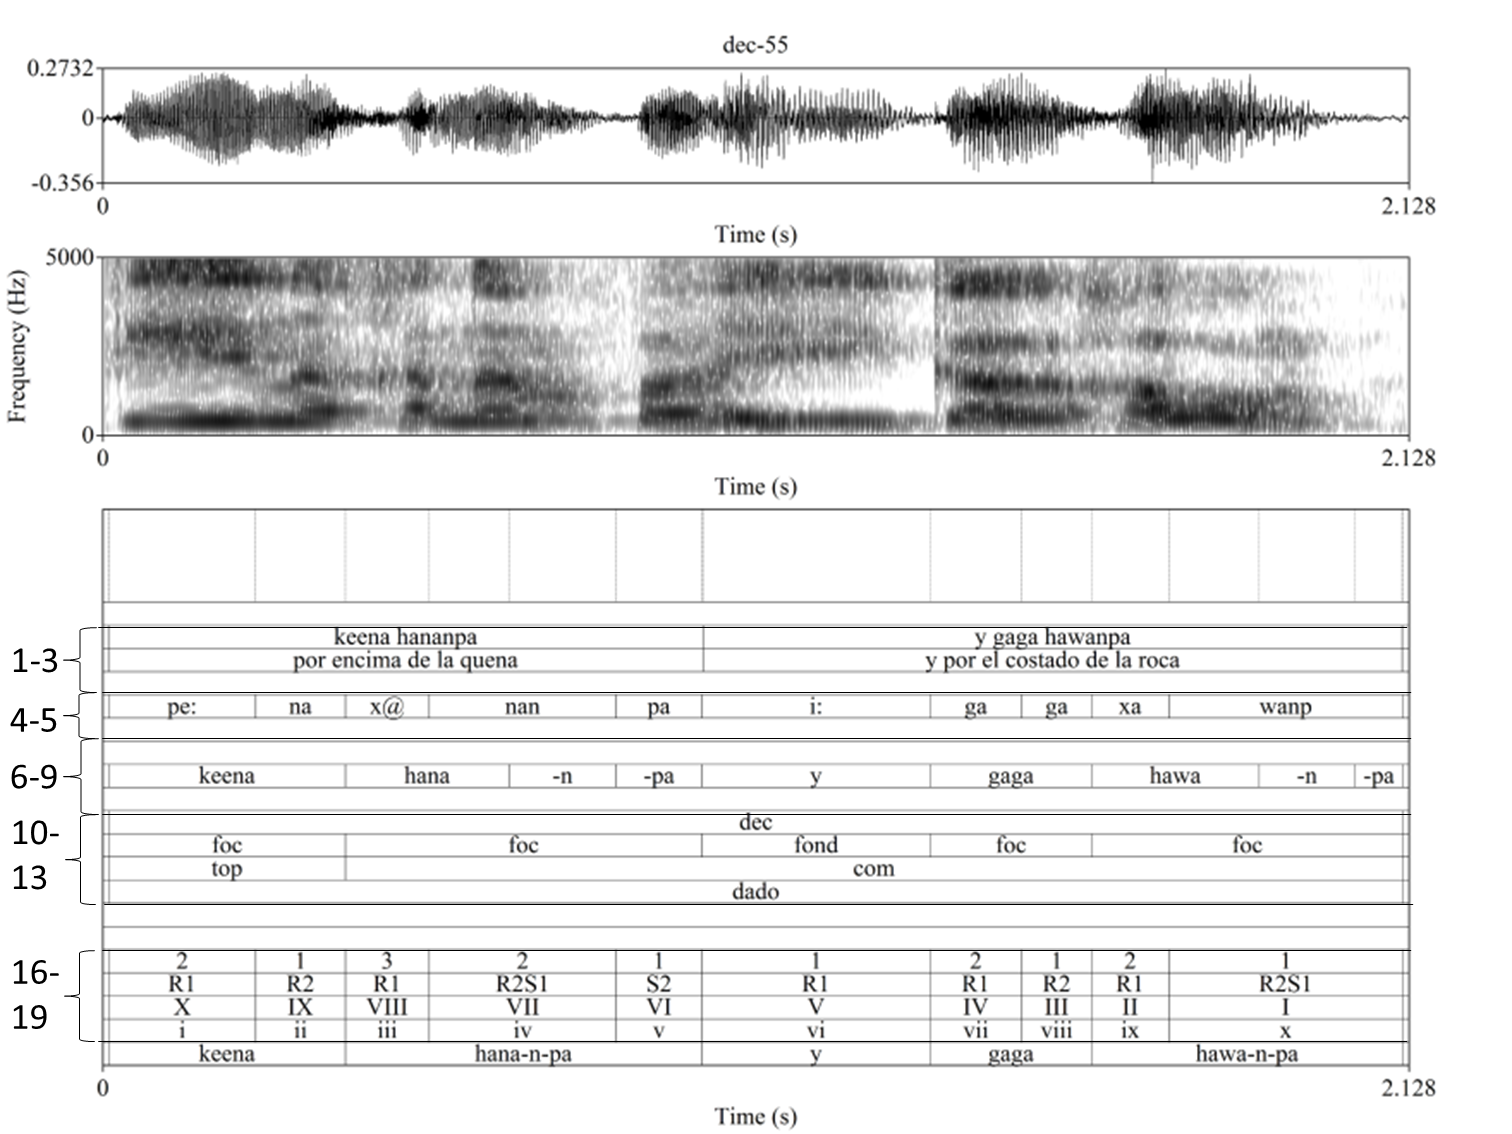
\includegraphics[width=\textwidth]{figures/BUC-img1small_numbered.png}
\caption{Waveform, spectrogram and text grid of the utterance \textit{keena hananpa y gaga hawanpa}.}
\label{fig:buc:1}
\end{figure}


%\begin{sidewaystable}
%\begin{tabularx}{\textwidth}{lSSSSSSSS}
%\lsptoprule
%Unit & N of boundaries (automatic version) & N of boundaries (revised version) & Correct boundaries & Moved boundaries & Deleted boudaries & Added boundaries & Percentage of correct boundaries (automatic version) & Percentage of actual boundaries correctly predicted \\
%\midrule
%Syllables & 1574 & 1574 & 1574 & 0 & 0 & 0 & 100 & 100 \\
%Stress groups & 628 & 628 & 543 & 85 & 0 & 0 & 86.46 & 86.46 \\
%Intonation groups & 354 & 323 & 274 & 31 & 49 & 18 & 77.40 & 84.82 \\
%Phonic groups & 168 & 168 & 168 & 0 & 0 & 0 & 100 & 100 \\
%\lspbottomrule
%\end{tabularx}
%\caption{Values for relative parameters in words of all lengths, counting from the right word boundary (see \figref{fig:buc:2})}
%\label{tab:buc:1}
%\end{sidewaystable}

This was done to avoid illusions of perfect \isi{phonetic} transcribability of spontaneous data on the one hand and to facilitate categorizations using these classes in the analysis on the other. Thus, in the example in \figref{fig:buc:1}, what is morphophonologically written in \REF{ex:buc:6}

\ea
\label{ex:buc:6}
\gll ke\textipa:na hana-n-pa i  gaga hawa-n-pa\\
flute above-\textsc{3s}.\textsc{poss}-\textsc{gen} and rock below-\textsc{3s}.\textsc{poss}-\textsc{gen}\\
\glt above the flute and below the rock
\z

\noindent is transcribed as in \REF{ex:buc:7}.

\ea
\label{ex:buc:7}
\ttfamily  <pe\textipa:{\textbar}na{\textbar}x@{\textbar}nan{\textbar}pa{\textbar}i\textipa:{\textbar}ga{\textbar}ga{\textbar}xa{\textbar}wanp>
\z

Voiceless plosives are transcribed with \texttt{<p>}, back fricatives [x ɣ h] with \texttt{<x>}, all nasals with \texttt{<n>}, reduced vowels with \texttt{<@>}, etc. Note that a phonetically somewhat more accurate rendering of the part transcribed as \texttt{<x@nanpa>} would be [xənampa]. Another remark needs to be made regarding \isi{syllable structure}. Note that in the transcription of /hawa-n-pa/, as opposed to /hana-n-pa/, \texttt{<wanp>} has been grouped as one \isi{syllable}, with a \isi{syllable structure} of CVCC, something which has not been described in the existing phonologies of \ili{Quechua} varieties (cf. \citealt{Parker1976} where a maximal \isi{syllable} is either CVC or CV\textipa:). This is because of the complete elision of the \isi{vowel} /a/ of the genitive marker \textit{-pa} in this case, as can also be seen on the spectrogram in \figref{fig:buc:1}, where there is no visible release of the plosive in the part corresponding to \texttt{<wanp>} as opposed to the plosive in the part corresponding to \texttt{<nanpa>}. This elision of vowels (as well as their sometime reduction) is a very frequent phenomenon in our variety of \ili{Quechua}, occurs both utterance-finally and –medially and is not restricted to this particular morpheme (which can also be realized fully). Note that we transcribed what was spoken and not any assumed underlying forms. 

Tiers 6--9 in the textgrid are used for a \isi{morphological annotation} and glosses (two tiers for each speaker). Whereas the syllabic transcription is a reduced transcription of the actual realization, the \isi{morphological annotation} represents morphemes in a form close to standard descriptions. Interval boundaries in the morphological tiers were made to coincide as closely as possible with the corresponding sound changes in the speech signal, however this was not always possible: a frequent example involves the copula \textit{ka-} together with the progressive \textit{-yka-}, as in 

\ea
\gll ka-yka-n\\
\textsc{cop}-\textsc{prog}-\textsc{3s}\\
\glt `S/he is in the process of being/having.'
\z
%\todo{suggest `S/he is in the process ...' done ur 0709}

Here the usual (but not the only) realization is  [ke\textipa:kan], %\todo{\isi{phonetic} : should probably be ː done 070917 ur} 
arising from a regular process of monophtongization in many central \ili{Quechua} varieties, thus making it impossible to determine where in the speech signal the boundary between the root and the progressive suffix lies. In such cases, labels on the morphological tier received a \texttt{<?>} after or before the connecting hyphen in the annotation. 

\subsubsection{Information structural annotation}
\label{sec:buc:3.3.2}
As can be seen from \figref{fig:buc:1}, the next four tiers in the annotation textgrid are used for information structural pragmatic categories. %\todo{suggest adding a table with columns for abbrevation; spanish; english; ur070917: See what you mean, will do that}
Tier 10 annotates the \isi{speech act}, with the categories \textsc{dec} for declaratives, \textsc{pregq} for queries, 
\textsc{pregch} for checks and \textsc{imp} for imperatives. 
Tier 11 is used for the annotation of focus-background structure, with \textsc{foc} for focus and \textsc{fond} for background. 
Tier 12 annotates topic-comment structure, with \textsc{top}, topic, and \textsc{com}, comment; 
tier 13 annotates givenness in the discourse with the categories of \textit{dado} `given', and \textit{nuevo} `new'. These annotations were made based on judgments about what role the parts of the utterance in question played in the discourse, not based on the presence or absence of morphological markers that have been described as encoding information structural meaning in \ili{Quechua} (cf. e.g. \citealt{Woelck1972,Weber1986,Muysken1995,GomezRendon2006}). Building on standard approaches to \isi{pragmatics} and \isi{information structure} (\citealt{Austin1962,Searle1969,Chafe1976,Bolinger1989,Rooth1992,Grice1997,Baumann2006,Krifka2007}, among many others) we elaborated the following set of key notions:  

%\todo{added small capitals for the defined terms; ur070917: cool, thank you}
\begin{itemize}
\item A \textsc{declarative} is adding a proposition to the common ground, regardless of whether this proposition is claimed by the speaker to be true (asserted) or not.
\item A \textsc{query} asks for information needed to complete a proposition, whether regarding its components (constituent question) or its truth value (polar question).
\item A \textsc{check} asks for confirmation that a proposition in the common ground should be considered to be true in the relevant world of discourse.
\item An \textsc{imperative} represents a command by the speaker (to the hearer) that a certain state of affairs in the world should be changed so as to conform to a proposition.
\item In \textsc{focus} are those parts of an utterance to which alternatives are saliently evoked and discarded; those which make a difference to propositions about states of affairs already in the common ground.
\item Correspondingly, in the \textsc{background} are those parts of an utterance to which alternatives are not evoked, that are not in focus; background is complementary to focus. 
\item \textsc{topic} is that part of a discourse that is currently being talked about or advanced by one of the participants in the discourse to be talked about henceforth, it is the frame of reference under which comments are to be understood. 
\item \textsc{commentary} is that which is talked about the topic; it is information that is added to the common ground regarding the topic. 
\item \textsc{given} are referents that are active in the discourse, whether they have been activated by linguistic or extralinguistic means. 
\item \textsc{new} are referents newly introduced into the discourse, they become active through their first (linguistic or extralinguistic) mention. 
\end{itemize}

These definitions are not without their problems: in particular, there exist certainly many more types of \isi{speech act} than just the four defined above; new and given are categorical impositions on a multitude of states of discourse activation that probably should be thought of as forming a graded scale; different types of focus such as information focus and \is{focus!contrastive}contrastive focus can and have been argued for (for a proposed hierarchy of them see \citealt{Fery2013}), and it is probably useful to further divide background into tail and link, as proposed by \citet{Vallduvi1992}. However, this part of the annotation is complex enough as it is, and we therefore decided to restrict ourselves to the above-mentioned categories, believing that they should suffice for the time being for the purposes of determining the relevance of information structural categories for the realization of \isi{prosody} in our data. 

These categories encode related but clearly distinct notions. Interactions may arise, e.g. when a new topic is introduced into the discourse it will often be in focus because it is then that it is contrasted with other alternatives. However, once it is introduced and well known, it is frequently not mentioned anymore, but the comments made about it are still divided between focus and background. This is only to make the point that the two are neither complementary nor the same, nor are any of the other categories defined above and annotated in separate tiers the same. We hold that it is not possible to further reduce these categories, such as they are defined above, without severely limiting one’s descriptive power and hence the scope of phenomena one would like to explain. 

It has only been possible to annotate these information structural categories in such comparative detail and on the basis of only discourse pragmatic considerations because the annotators both also designed the experiments that produced the semi-spontaneous data (controlling a large percentage of the content words metrically) and were present during the course of the experiments as silent participants. Thus both the states of affairs that are talked about as well as the (linguistic and extralinguistic) discursive progression of events are well known to us, and our annotations (of course remaining interpretations to a certain degree, but this is valid for all annotations) are anchored in and informed by these facts. 

\subsubsection{Positional annotation}
Tiers 16--19 in \figref{fig:buc:1} demonstrate what we call \isi{positional annotation}. In order to create the intervals, a {Praat} script first cut the entire map task recording with its textgrid into chunks at the \isi{speech act} grid that correspond roughly to conversational moves and are surrounded by (small) silences. Another script then detected in which of the two \isi{syllable} tiers, annotating the two speakers respectively, there were more intervals and made four empty copies of its intervals in tiers 16--19, thus selecting only the more dominant speaker for each such chunk to be analyzed. In most cases, this yielded sound-textgrid pairs without any speaker overlap. In those cases where there was speaker overlap, the parts where the less dominant speaker was speaking were excluded from the analysis. The intervals in tiers 16--19 were then labelled as follows, creating the \isi{positional annotation}:

Tier 16 annotates \isi{syllable position} in the word counting from its right edge, using Arabic numerals (1, 2, 3, 4, etc.). Thus, in the example given and starting from the right, the \isi{syllable} \texttt{<wanp>} receives in its corresponding interval on tier 16 a <1>, \texttt{<ha>} a <2>; the right \texttt{<ga>} from \textit{gaga}, because it is a separate word, again receives a <1>, and to its left the other \texttt{<ga>} a <2>. “Word” here refers to the morphological word in \ili{Quechua} whose structure all grammars agree upon, i.e. consisting of a root plus several suffixes. Theoretically, due to the agglutinative nature of \ili{Quechua}, any number of suffixes could be attached to a root; in practice, the furthest a \isi{syllable} was annotated as being removed from the \isi{right word boundary} in this corpus was 6, and 3 was not often exceeded. The implicit assumption here is that the domain of the morphological word is largely isomorphic with a relevant \isi{prosodic domain}, e.g. the \isi{prosodic word} in \ili{Quechua}, if it exists, although this is in fact unknown. Note that what is annotated here are syllables as defined in the part on \isi{syllable} transcription and transcribed in tiers 4 and 5, not morphemes.\largerpage[-1] 

Tier 17 annotates \isi{syllable position} in the word counting from its left edge as well as morphological category (root or suffix). The labeling consists of either “R”, for root, or “S”, for suffix, plus an Arabic numeral indicating position and whose counting is reset at the border between root and suffix. To clarify using the example from figure \ref{fig:buc:1}: Starting from the left, \texttt{<pe\textipa:>} and \texttt{<na>} are labelled <R1> and <R2> respectively, because they are both part of the root of the verb. Proceeding, \texttt{<x@>}, as the first \isi{syllable} of the next word, gets labelled <R1> again, but \texttt{<nan>}, because it consists both of the second part of the root \textit{hana-} `above' and the first suffix \textit{-n} ``3\textsuperscript{rd} singular possessive'', is labelled <R2S1>. With this twofold annotation, it is possible to examine both position from left-edge \isi{word boundary} and whether a \isi{syllable} is part of the root or the suffixes of a word as influencing factors on \isi{prosody} in the later analysis.      

Tier 18 annotates \isi{syllable position} in the whole utterance counting from its right edge using large Roman numerals (I, II, III, IV, etc.). The utterance is here defined as consisting of what is labelled as one conversational move between (short) pauses, hence everything one speaker says “in one go”. This may correspond in many cases to a \isi{prosodic} phrase, if only to postulate a \isi{prosodic domain} distinct from the word in \ili{Quechua}. Whether this phrase is in itself composed of further smaller phrases that are not isomorphic with the (postulated) \isi{prosodic word} in \ili{Quechua} is not known (see \citealt{Grice2000} for discussion of the concept). To look at the example, the interval on tier 18 corresponding to the \isi{rightmost syllable} \texttt{<wanp>} is labelled with a <I>, from there the numbering increases rightward until the interval corresponding to the \isi{leftmost syllable}, <pe\textipa:>, which gets labelled \texttt{<X>} for being the tenth \isi{syllable} in the entire phrase counting from the right. 

Tier 19 works exactly as tier 18, only counting from the left edge of the utterance/phrase and with the numbering being done in small Roman numerals (i, ii, iii, iv, etc.). Thus, the \isi{leftmost syllable} <pe\textipa:> here gets labelled <i>, and \texttt{<wanp>} at the right edge <x>, for being the tenth \isi{syllable} in the phrase if counting from the left. 

Proceeding in this way has several advantages: Only by using four tiers for positional measurements can we exactly observe and quantify \isi{prosodic} behavior at both the left and the right edge of two domains, that of the word and that of the phrase. Note that none of the tiers annotates information already given in another tier; since both word length and phrase length are highly variable, the left-counting tiers can only give precise positional information at the left edge of the domain, and vice versa for the right-counting ones. This procedure incorporates standard assumptions in every theory of metrical phonology (e.g. \citealt{Liberman1977,Hayes1995}; \citealt{Hulst1999}).\footnote{If our method were to show that no kind of \isi{prominence} is computable from the edges we would have to assume \isi{prominence} as a diacritic in the \isi{phonological word} in \ili{Quechua}. This is hard to believe. Rather, we expect some aspects to be derived metrically and others to be lexically fixed.} Since it is so far unknown which \isi{prosodic} domains play a role in \isi{prominence} assignment in \ili{Quechua}, it would be inadvisable to neglect one of these domains by not annotating for syllabic position in it. On the other hand, if the later analysis shows consistent results e.g. in the \isi{prosodic} behavior of syllables counted from the right edge of the phrase but not the word, it will be possible to conclude that this domain definitely does play a role. We think that the domains annotated as they are here are the best possible candidates so far for playing a role in influencing \isi{prosodic} phenomena and only after the final analysis will it be possible to see where they need to be further refined.  

To complete the description of the annotation process, there is also a derivative tier of the morphological tier, tier 20, that annotates word-length elements by copying the tier of the \isi{morphological annotation} and leaving only those boundaries that are to the left of the beginning of the root of a word (using information from tier 17). A script in {Praat} was written for that and the results checked. This helps to take important measurements in relation to word length, an information that wasn’t contained in the textgrid up to that point, as will be seen in the next section.       

\subsection{Measurements} 
A {Praat} script was written that used the information encoded in the annotation textgrids detailed above. Per annotated \isi{syllable}, it was used to extract the relevant annotational information from the tiers in the textgrid described above, i.e. what word the \isi{syllable} belongs to, which one of the two speakers is uttering it, what information structural categories it is annotated for, what position according to the positional annotations it has, etc. Acoustic measurements per \isi{syllable} were also taken by it from the sound files in the corpus. The measurements taken can be divided into two kinds: absolute and relative.

\subsubsection{Absolute measurements} 
We extracted measurements of F0, intensity and duration, all of which have been shown to variously play a role in the encoding of \isi{prominence}. In particular, the absolute measurements taken were:

\begin{enumerate}
\item  Syllable duration in ms
\item  Mean F0 per \isi{syllable} in Hz
\item  Minimum F0 per \isi{syllable} in Hz
\item  Maximum F0 per \isi{syllable} in Hz
\item  Position of minimum and maximum F0 within the \isi{syllable}
\item  Pitch range within the \isi{syllable} in Hz
\item  Mean intensity per \isi{syllable}
\end{enumerate}

From the measurements for F0 minimum and maximum, the script further created a categorical measurement of F0 movement for each \isi{syllable}: if minimum and maximum were at least 30\,Hz and 100\,ms (about one standard deviation of the \isi{syllable duration} in the sample) apart from each other, the \isi{syllable} would be assigned one of the labels “rising” or “falling”, depending on whether the movement was from minimum to maximum or the other way round; if these criteria were not met, the \isi{syllable} was assigned the label “level”.  

\subsubsection{Relative measurements}
\label{sec:buc:3.4.2}


The relative measurements are based on the deliberation that \isi{prominence} by definition is a relative concept. It is impossible to make a statement about the \isi{prominence} of a \isi{syllable} just from knowing that e.g. it has a certain mean F0 value or even that it has a large \isi{pitch range}, without a comparison with the corresponding values of other units, i.e. that of adjacent syllables or the mean value of the word the \isi{syllable} is a part of. That is exactly what the relative measurements do (for a similar approach, see \citealt{PamiesBertran1996}). For most of the absolute measurements, the script also produces relative values that serve as a comparison with the corresponding acoustic parameter on three levels: that of the adjacent \isi{syllable} (left and right if they exist, i.e. if the \isi{syllable} isn’t itself at a domain edge), that of the word, and that of the phrase (each as defined within the annotation method described above). These are the relative measurements obtained per \isi{syllable}:

\begin{enumerate}
\item  Syllable duration divided by average \isi{syllable duration} within the phrase
\item  Syllable duration divided by average \isi{syllable duration} within the word
\item  Syllable duration divided by duration of the \isi{left-adjacent syllable} (if it exists)
\item  Syllable duration divided by duration of the right-adjacent \isi{syllable} (if it exists)
\item  Mean F0 of the \isi{syllable} divided by mean F0 of the phrase
\item  Mean F0 of the \isi{syllable} divided by mean F0 of the word
\item  Mean F0 of the \isi{syllable} divided by mean F0 of the \isi{left-adjacent syllable} (if it exists)
\item  Mean F0 of the \isi{syllable} divided by mean F0 of the right-adjacent \isi{syllable} (if it exists)
\item  Pitch range of the \isi{syllable} divided by \isi{pitch range} of the \isi{left-adjacent syllable} (if it exists)
\item  Pitch range of the \isi{syllable} divided by \isi{pitch range} of the right-adjacent \isi{syllable} (if it exists)
\item  Mean intensity of the \isi{syllable} divided by mean intensity of the phrase
\item  Mean intensity of the \isi{syllable} divided by mean intensity of the word
\item  Mean intensity of the \isi{syllable} divided by mean intensity of the \isi{left-adjacent syllable} (if it exists)
\item  Mean intensity of the \isi{syllable} divided by mean intensity of the right-ad\-ja\-cent \isi{syllable} (if it exists)
\end{enumerate}

A few remarks need to be made regarding these measurements. In general, the script was written so as to recognize when a \isi{syllable} had no left- or right-adjacent \isi{syllable}, so it wouldn’t take the corresponding relative measurement. Then, because they are obtained by dividing the value of a parameter for the \isi{syllable} that is being investigated by the corresponding value of another unit, all of these relative measurements are naturally grouped around the value 1 in the sense that if they are larger than 1, it means that the value of the \isi{syllable} in question is higher than that of the unit it is compared with; if it is below 1 it is lower than that of the other unit in comparison; if it is exactly 1 the two values compared are the same. These values increase exponentially, therefore their log-10s were taken so that they are now grouped around 0, increase linearly and statistical measurements such as means can be applied to them. 

Note that we originally intended to also compare formant measurements between syllables in order to look at \isi{vowel} reduction as a correlate of non-pro\-mi\-nence. However, implementing this would not be straightforward, as only phonologically same vowels that are adjacent could be reasonably compared, and then only via a derived measure comparing e.g. distance between F1 and F2, as an indicator of centralization of the \isi{vowel}. However, centralization is not the only way of reducing vowels,\footnote{Note that in two studies on (unstressed) \isi{vowel} reduction in Cusco \ili{Spanish} \citep{Delforge2008} and \il{Quechua!Cusco}Cusco Quechua \citep{Delforge2011}, the phenomenon is described as existent and wide-ranging but consisting phonetically of instances of \isi{vowel} devoicing with no apparent centralization. While this might well be the case, the fact that \il{Quechua!Cusco}Cusco Quechua and the Central \ili{Quechua} varieties are so different in many other respects means that we are unwilling to simply transfer these conclusions to our case. Besides, \citet{Delforge2011} never connects \isi{vowel} reduction in \ili{Cusco Quechua} with any \isi{prosodic} properties of the language, so that the relation between \isi{vowel} reduction and stress or \isi{accent} in \ili{Quechua} remains entirely unexplored so far.} so this would still be an insufficient procedure. We decided to exclude \isi{vowel} quality from the scope of this preliminary study and to perform a detailed analysis of it later. 

\subsection{Putting things into interaction}
A total of 1019 syllables of the pilot corpus were annotated and measured in the way described above. 26 of these had to be excluded because of overlap between speakers, reducing the number of syllables that can be used in the analysis to 993. After applying the steps described above, there are now per \isi{syllable} up to 43 numerical (ratio and interval) variables obtained through the acoustic measurements and 12 categorical (nominal and ordinal) variables obtained by extraction of the relevant annotation information from the textgrid. A further categorical variable, \isi{syllable} type (C, CV, V\textipa:, CVC etc.), was derived from the \isi{syllable} annotation by using regular expressions in {R} (\citealt{Rtool}). Now, the purpose of this approach is to bring to light the effect each of the linguistic categories encoded in the annotation has on \isi{realizational strength}, which is supposed to encode phonological \isi{prominence}. For this purpose, the data was imported into {R}, so that the measurements could be plotted in dependence on the categorical variables, either in isolation or in conjunction. There are two important points to consider. The first is that in our pilot corpus, we do not have a balanced sample with regards to frequency of occurrence of the variants the categorical variables may assume. That is, if we were to compare the mean values of the \isi{rightmost syllable} in the word with that of the fifth \isi{rightmost syllable} in the word just like that, the results would be skewed, because there are just 15 syllables in the corpus that are annotated as being in the fifth rightmost position of the word, whereas there are 410 syllables in rightmost position within the word. The same would happen when comparing declaratives with imperatives; while there are more than 600 syllables annotated as belonging to the former category, there are only 15 for the latter. Differences in variance between the two groups to be compared would result more from the differences in sample size than from any inherent properties of the underlying populations. Ideally we would need a much larger sample, so even rarer variants and conditions would still have enough occurrences to allow for a meaningful comparison. Since this is not feasible with the sample size we have, a preliminary solution must be to exclude rare variants and to only work with those that have a reasonable number of occurrences in the dataset. The second point is related, but of a more linguistic nature. When comparing measurements, again, between the rightmost, the second rightmost and the third \isi{rightmost syllable} of a word, the results will be of little value if care isn’t taken to make sure that the second and third rightmost syllables aren’t sometimes initial syllables, a fact that might influence \isi{prosodic} realization. In other words, it makes more sense to compare syllables belonging to words of the same length. 

\subsection{The realizational coefficient} 
One approach that is interesting to pursue exploits the nature of the relative measurements taken. Since they are all (log-10s of) ratios of a parameter measured for one \isi{syllable} to that of an adjacent (left or right) \isi{syllable} or larger unit, they are all at the same scale and therefore comparable. They can also be used in combination. Adding together relative values for one measurement with those of another and dividing by their number, we get average ratios per \isi{syllable} of several parameters at once. For example, we can get an overall realizational value for the ratio of one \isi{syllable} to its adjacent syllables by taking the relative values of \isi{syllable duration} divided by that of its left- and right-adjacent syllables, as well as those for mean F0, \isi{pitch range} and intensity, adding them together and dividing them by the number of values added (eight in this case). Since these values express relative \isi{realizational strength} of one \isi{syllable} over others, we may name the result (somewhat tongue-in-cheek) the overall realizational coefficient(s). With the help of these coefficients we can determine the relative \isi{realizational strength} of any \isi{syllable position} in our data, as well as (by comparison with the singular relative measurements) its contributing factors. Thus it is possible to show not only why a certain \isi{syllable position} is strong when viewed e.g. at the word level, and what parameter is responsible for this, but also why it might not be very salient at another level (e.g. the phrase level), for example because the effect one parameter has at one level is overruled by that of another at another level. It needs to be pointed out that the same coefficients cannot always be used equally. Syllables at phrase edges have empty pauses to one of their sides, and the {Praat} script did not take relative measurements for them towards that side, see \sectref{sec:buc:3.4.2}. For that reason, when looking at phrase-level measurements, the values comparing syllables with average \isi{syllable} values in their phrase were used. In theoretical terms, using these realizational coefficients will help us to disentangle the interaction of the different means of creating \isi{prominence} at different levels.

\section{Preliminary results}
In the following, some of the findings resulting from looking at the measurements at the different \isi{syllable} positions under some of the information structural conditions will be presented and discussed. The purpose is here to explore the capabilities and limitations of the method described for creating profiles of realizational \isi{prominence} in the data. In order to gain a comprehensive overview of the multidimensional dataset, hundreds of combinations of conditions were examined in different ways. We can only report on a few of the ones that seem to be most promising for future exploration. Since the sample is not balanced, we decided not to use any inferential statistics in order not to create false impressions of the general validity of our results unsuitable to the exploratory nature of this study. 

\subsection{Prominent syllables: Penultima}
One important overall finding that derives from several ways of looking at the data is that the \isi{penultimate syllable} is indeed prominent in the sense that something is happening there, but that it isn’t at all certain that the \isi{prosodic domain} of which this is the \isi{penultimate syllable} is really isomorphic with the word as defined here. To explore this finding in more detail, let us proceed from looking at overall values to more individual ones:

\figref{fig:buc:2} shows barplots of the median values obtained for the first four \isi{syllable} positions in the word (we left out the fifth and sixth due to small token size and better visibility) counted from the \isi{right word boundary}, for the whole dataset used. The ends of the bars indicate the (medians of the) ratio of the parameter measured for the respective \isi{syllable position}, divided by its immediate neighbours to the left and right (where applicable). The parameters used are mean F0 per \isi{syllable} (red), \isi{pitch range} (orange), duration (blue), intensity (green) and all four combined and divided by their number (black, from here on called ``the left-right overall coefficient", see above). Considering the left-right overall coefficient, the \isi{penultimate syllable} of the word obtains median (0.0081) and mean (0.0072, sd=0.1197) values only slightly above zero (meaning that at least half of its values are better than those of its adjacent syllables). Almost all other \isi{syllable} positions also have median values slightly above zero, and their quartiles (see \tabref{tab:buc:1}) range very far both below and above zero. Hence the penult is not particularly \textit{more} prominent in this regard than other positions. The values for the left-right overall coefficient are very small here, even compared to the already small scale used in this figure.\footnote{%
\begin{samepage}
It has to be borne in mind how these graphs are to be read: the values on the y-axis are logarithms of base-10 (log-10) of the ratio of a value obtained in a parameter for a \isi{syllable} in the indicated position divided by the values obtained for the same parameter by either its adjacent syllables or the larger unit (word/phrase), thus representing relative \isi{realizational strength} of the \isi{syllable} in that parameter (see \sectref{sec:buc:3}). A value of zero on the y-axis therefore means that the \isi{syllable} is equally strong in the parameter as the unit it is compared with, positive values mean that it is realizationally stronger relative to the compared unit, negative values mean that it is weaker. A log-10 value of 0.1 corresponds to a ratio of about 1.259:1 (meaning that the value for the \isi{syllable} is about 25\,\% higher than that of the unit it is compared with), a log-10 value of 0.04 to a ratio of ~1.096:1 (a little less than 10\,\% higher), a log-10 value of 0.02 to a ratio of ~1.047:1 (a little less than 5\,\% higher), a log-10 value of 0 to a ratio of 1:1, a log-10 value of -0.02 to a ratio of ~0.955:1 (a little less than 5\,\% below the value for the compared unit), a log-10 value of -0.04 to a ratio of ~0.912:1 (a little less than 10\,\% below), and a log-10 value of -0.1 to a ratio of 0.794:1 (a little more than 20\,\% below), and so on, to give an example. The barplots indicate the median value for each \isi{syllable position}. Each individual measurement obtained above zero means that this \textit{individual} \isi{syllable} is more realizationally strong in the parameter measured than its \textit{specific} \textit{and individual} neighbors. A median above zero thus means that this is the case for at least half of all syllables in this position. Because of the lower quartiles reaching below zero (see \tabref{tab:buc:1}) and the differing token sizes per \isi{syllable position}, there is no contradiction with several positions having their medians above zero: this only means that there is a smaller percentage of syllables that are less realizationally strong than their individual neighbors.
\end{samepage}
}
This reflects the fact that the parameters it is composed of do not show a uniform pattern, i.e. do not unequivocally indicate a \isi{prominence} for the penult at all. For example, the penult actually has a median slightly below zero for the parameter of duration, and at zero for the parameter of \isi{pitch range}. Duration seems to instead favour the anteantepenult and \isi{pitch range} the ultima, and also for mean F0, the median values for the penult do not stand out particularly from those of the antepenult. Hence, the picture we get from this very first approach to the data is less than unified, and does not seem to indicate a state of affairs in which all acoustic parameters unite in order to make a single \isi{syllable} in the domain of the \isi{prosodic word} stand out from all others. Taking a look at specific conditions, word lengths and the individual realizational parameters will hopefully provide more detailed insight.

\begin{figure}
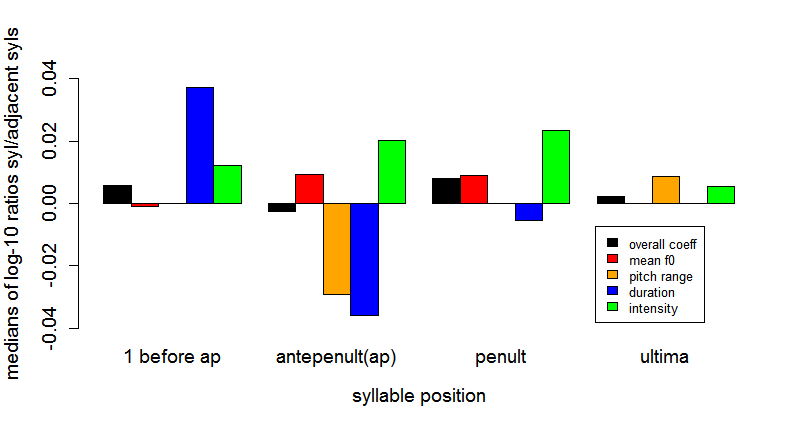
\includegraphics[width=\textwidth]{figures/BUC-img2_new.png}
\caption{Barplots comparing the medians of 5 log-10 ratios obtained by dividing the value for the syllable by that of its adjacent syllables in the word, ordered according to syllable position in the word from the right word boundary: the overall (black), mean F0 (red), pitch range (orange), duration (blue) and intensity (green) left-right coefficients for the entire sample. N (1 before antepenult) = 49; N (antepenult) = 136; N (penult) = 281; N (ultima) = 255}
\label{fig:buc:2}
\end{figure}


\begin{sidewaystable}

\begin{tabular}{ll *{5}{S[table-format=1.8,group-digits=false]}r}
\lsptoprule
\pbox{1.6cm}{type of coefficient} & \pbox{3.2cm}{\isi{syllable position} in word} & \pbox{1.7cm}{lower quartile} & \multicolumn{1}{c}{median}     & \multicolumn{1}{c}{mean}       & \pbox{1.7cm}{upper quartile} & \multicolumn{1}{c}{sd}         & \pbox{1.6cm}{N tokens (syllables)} \\
\midrule
overall                                                         & 3 before antepenult       & -0.09176       & -0.06776   & -0.06776   & -0.04375       & 0.06790292 & 2                            \\
                                                                & 2 before antepenult       & -0.05519       & 0.02811    & 0.01336    & 0.05518        & 0.08698023 & 11                           \\
                                                                & 1 before antepenult       & -0.04438       & 0.00570    & 0.01235    & 0.07184        & 0.10113552 & 49                           \\
                                                                & antepenult                & -0.061365      & -0.002598  & -0.007605  & 0.048850       & 0.10058366 & 136                          \\
                                                                & penult                    & -0.059410      & 0.008110   & 0.007206   & 0.078412       & 0.11970251 & 281                          \\
                                                                & ultima                    & -0.061826      & 0.002242   & 0.003760   & 0.083105       & 0.12473560 & 255                          \\
\midrule                                                                
mean f0                                                         & 3 before antepenult       & -0.032162      & -0.021081  & -0.021081  & -0.010000      & 0.03134178 & 2                            \\
                                                                & 2 before antepenult       & -0.003155      & 0.007354   & 0.007931   & 0.027405       & 0.04696297 & 11                           \\
                                                                & 1 before antepenult       & -0.0319673     & -0.0009873 & -0.0057637 & 0.0106195      & 0.04610146 & 49                           \\
                                                                & antepenult                & -0.009671      & 0.009344   & 0.006082   & 0.026019       & 0.05388791 & 136                          \\
                                                                & penult                    & -0.007283      & 0.008938   & 0.006025   & 0.031923       & 0.05610093 & 281                          \\
                                                                & ultima                    & -0.025128      & -0.000083  & 0.002712   & 0.024209       & 0.08117007 & 255                          \\
\midrule
\isi{pitch range}                                                     & 3 before antepenult       & -0.37810       & -0.17418   & -0.17418   & 0.02975        & 0.5767830  & 2                            \\
                                                                & 2 before antepenult       & 0.0000         & 0.1431     & 0.1552     & 0.2426         & 0.3651206  & 11                           \\
                                                                & 1 before antepenult       & -0.19496       & 0.00000    & 0.07306    & 0.28384        & 0.4362566  & 49                           \\
                                                                & antepenult                & -0.35170       & -0.02925   & -0.06869   & 0.15508        & 0.4262779  & 136                          \\
                                                                & penult                    & -0.22749       & 0.00000    & 0.02314    & 0.28935        & 0.4921704  & 281                          \\
                                                                & ultima                    & -0.231225      & 0.008477   & 0.005969   & 0.316592       & 0.5207739  & 255                         \\
\lspbottomrule
\end{tabular}
\caption{Values for relative parameters in words of all lengths, counting from the right word boundary (see \figref{fig:buc:2})}
\label{tab:buc:1}
\end{sidewaystable}


\begin{sidewaystable}
\begin{tabular}{ll *{5}{S[table-format=1.8,group-digits=false]}r}
	\lsptoprule
	\pbox{1.6cm}{type of coefficient} & \pbox{3.2cm}{\isi{syllable position} in word} & \pbox{1.7cm}{lower quartile} & \multicolumn{1}{c}{median}     & \multicolumn{1}{c}{mean}       & \pbox{1.7cm}{upper quartile} & \multicolumn{1}{c}{sd}         & \pbox{1.6cm}{N tokens (syllables)} \\
	\midrule
duration            & 3 before antepenult       & -0.1461        & -0.1414   & -0.1414   & -0.1368        & 0.01308885  & 2                            \\
                    & 2 before antepenult       & -0.19105       & -0.05224  & -0.07615  & 0.06760        & 0.17805208  & 11                           \\
                    & 1 before antepenult       & -0.120304      & 0.037103  & 0.002385  & 0.151268       & 0.20698473  & 49                           \\
                    & antepenult                & -0.16943       & -0.03586  & -0.01976  & 0.11743        & 0.20664683  & 136                          \\
                    & penult                    & -0.169099      & -0.005398 & -0.016198 & 0.149812       & 0.24136864  & 281                          \\
                    & ultima                    & -0.158923      & 0.000000  & -0.003881 & 0.154910       & 0.23593383  & 255                          \\
\midrule
intensity           & 3 before antepenult       & 0.010245       & 0.012472  & 0.012472  & 0.014700       & 0.006300656 & 2                            \\
                    & 2 before antepenult       & -0.007806      & 0.016768  & 0.006260  & 0.022976       & 0.025963067 & 11                           \\
                    & 1 before antepenult       & -0.004430      & 0.012249  & 0.009791  & 0.023763       & 0.023103567 & 49                           \\
                    & antepenult                & 0.004583       & 0.020092  & 0.018961  & 0.035845       & 0.027377440 & 136                          \\
                    & penult                    & 0.009766       & 0.023370  & 0.022498  & 0.038142       & 0.025619751 & 281                          \\
                    & ultima                    & -0.010866      & 0.005356  & 0.001503  & 0.018054       & 0.027426937 & 255                         
\\
\lspbottomrule
\end{tabular}
\caption{Values for relative parameters in words of all lengths, counting from the right word boundary (see \figref{fig:buc:2})}
\label{tab:buc:2}
\end{sidewaystable}




\subsection{Word length} 
As explained above, by controlling for word length we eliminate possible effects of left-edge phenomena. If only words of the same length are compared, we can observe not only the right, but also the left edge of the word. The \isi{syllable position} that is leftmost in the graph is now also the \isi{leftmost syllable} in the word. Additionally, token sizes for each \isi{syllable position} are now equal (almost, because of elimination of syllables for reasons such as speaker overlap or being at the edge of the phrase). We can thus create more reliable \isi{prominence} profiles for each word length. Unfortunately, in this sample, this kind of reduction also means that we can only effectively observe words from lengths 2--4 (see token sizes given in the descriptions for the figures). 

\begin{samepage}

Both two-\isi{syllable} and three-\isi{syllable} words do not especially indicate \isi{prominence} for the penult (see Figure \ref{fig:buc:3}, comparing the left-right overall coefficient for words of length 2 (black), 3 (red) and 4 (blue)).  

\end{samepage}

\begin{figure}
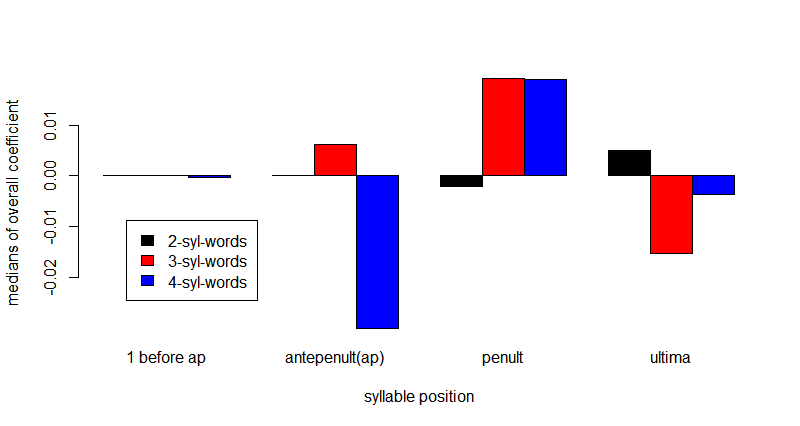
\includegraphics[width=\textwidth]{figures/BUC-img3_new.png}
 \caption{Barplots comparing the medians of the overall left-right coefficient for words of syllable length 2 (black), 3 (red) and 4 (blue), ordered according to syllable position in the word from the right word boundary. For 4-syllable words: N (1 before antepenult) = 31; N (antepenult) =  43 (4-syl words); N (penult) = 44; N (ultima) = 28. For 3-syllable words: N (antepenult) = 71; N (penult) = 110; N (ultima) = 72. For 2-syllable words: N (penult) = 105; N (ultima) = 116}
\label{fig:buc:3}
\end{figure}


%\begin{figure}
%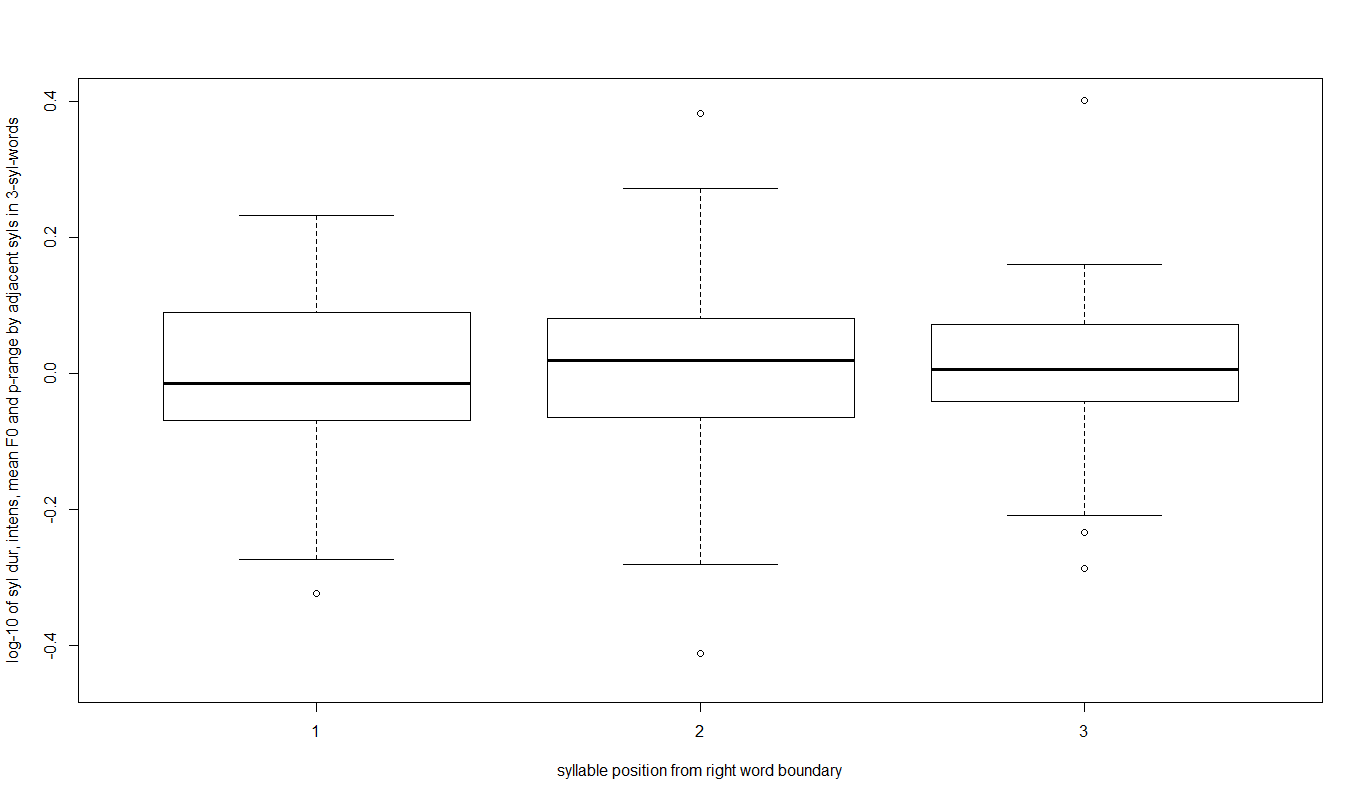
\includegraphics[width=\textwidth]{figures/BUC-img4.png}
%\caption{Boxplots of left-right overall coefficient by syllable position from the right word boundary, only words of syllable length 3. \\ N(1) = 72; N(2) = 110; N(3) = 71}
%\label{fig:buc:4}
%\end{figure}


The medians for all positions are more or less the same in 2-\isi{syllable} words, and in 3-\isi{syllable} words the median of the penult is the highest, but not by much. Not much indication, either, for a stronger realization of the \isi{initial syllable}. However, in 4-\isi{syllable} words, the picture changes (see \figref{fig:buc:3}). Here, the median of the penult is visibly higher than that of its surrounding positions.  

%\begin{figure}
%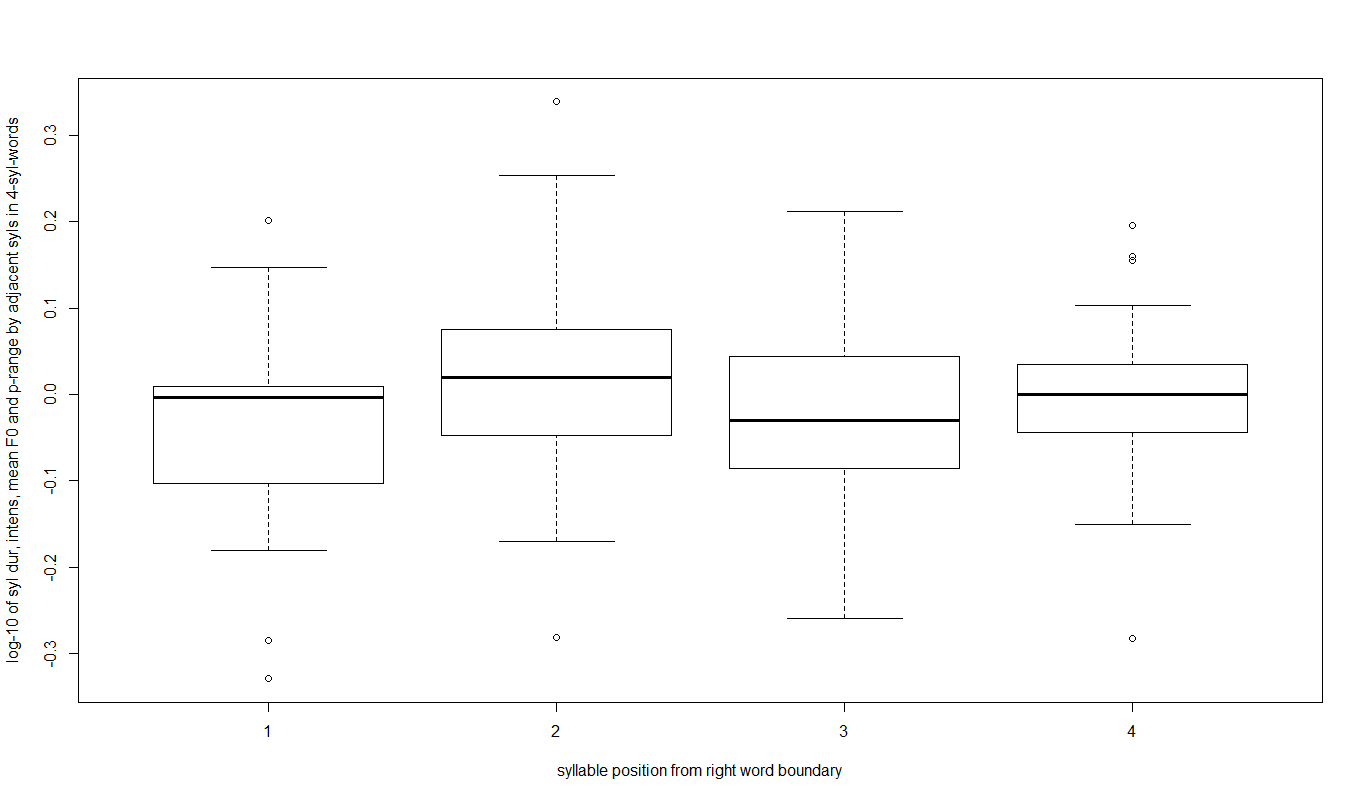
\includegraphics[width=\textwidth]{figures/BUC-img5.png}
%\caption{Boxplots of left-right overall coefficient by syllable position from the right word boundary, only words of syllable length 4. \\
%N(1) = 28; 
%N(2) = 44; 
%N(3) = 43; 
%N(4) = 31
%}
%\label{fig:buc:5}
%\end{figure}


The \isi{initial syllable} is also stronger in its realization than the ultimate and antepenult. This would give some support to the proposal of a primary \isi{prominence} on the penultimate, and a secondary \isi{prominence} on the initial or every second \isi{syllable} from it (which of the two cannot be determined here), or one where \isi{prominence} is assigned metrically to every second \isi{syllable} in a unit. It has to be kept in mind however, that the ratios obtained here are again very small overall, indicating differences in the \isi{realizational strength} of the syllables of at most 10--15\,\%.

\subsection{Different parameters}
We will now explore the factors contributing to the values of the overall realizational coefficient, i.e. the three acoustic parameters it consists of, duration, F0 and intensity. We will see how they support the finding of the \isi{penultimate syllable} receiving word-level \isi{prominence}. 

\subsubsection{F0}
There are several ways in which F0 can reasonably influence \isi{realizational strength}. Leaving other things aside, an interesting difference arises between the relative measurements of mean F0 per \isi{syllable} and \isi{pitch range} per \isi{syllable} divided by their adjacent syllables. See \figref{fig:buc:4} showing the values for \isi{pitch range} (dark blue) and mean F0 (red) per \isi{syllable}, both in words of length 4.

\begin{figure}
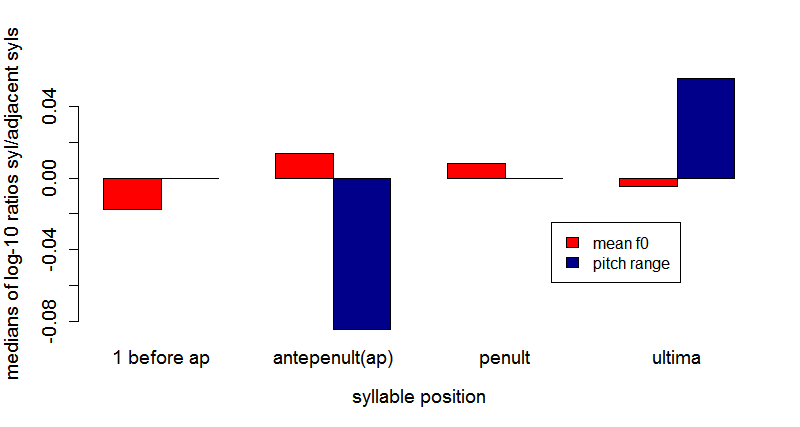
\includegraphics[width=\textwidth]{figures/BUC-img4_new.png}
\caption{
Barplots comparing the medians of the left-right  {pitch range} (dark blue) and mean F0 (red) coefficients for words of  {syllable} length 4, ordered according to  {syllable position} in the word from the  {right word boundary}. N (1 before antepenult) = 31; N(antepenult) = 43; N (penult) = 44; N (ultima) = 28
}
\label{fig:buc:4}
\end{figure}

%\begin{figure}
%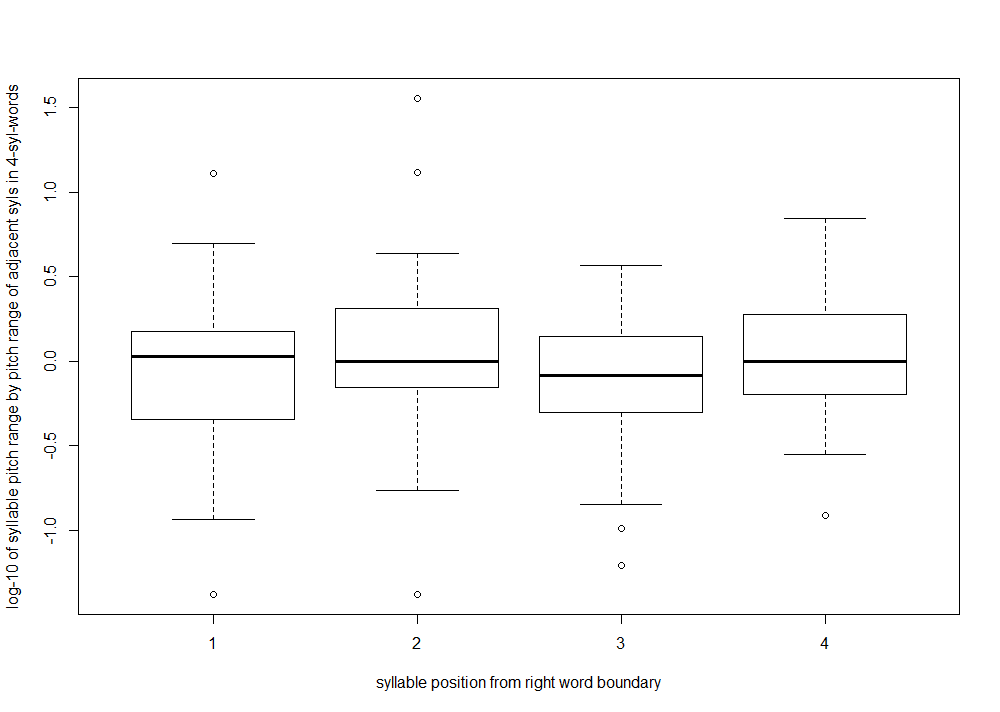
\includegraphics[width=\textwidth]{figures/BUC-img6.png}
%\caption{
%Boxplots of left-right \isi{pitch range} coefficient by \isi{syllable position} from the \isi{right word boundary}, only words of \isi{syllable} length 4. \\
%N(1) = 28; 
%N(2) = 44;
%N(3) = 43; 
%N(4) = 31
%}
%\label{fig:buc:6}
%\end{figure}


While the values for \isi{pitch range} seem to display an alternating pattern, with the ultima realizing the largest range in comparison with adjacent syllables, the antepenult the least, and the penult and \isi{initial syllable} being more or less equal, the values for plain F0 form a sort of arc, with low values at the edges and high ones in the two middle positions. These two results are what would be expected if the actual F0 pattern was that of a rise on the \isi{initial syllable}, a plateau on the intervening one(s), and a drop on the penult (and/or ultima, see below).

%\begin{figure}
%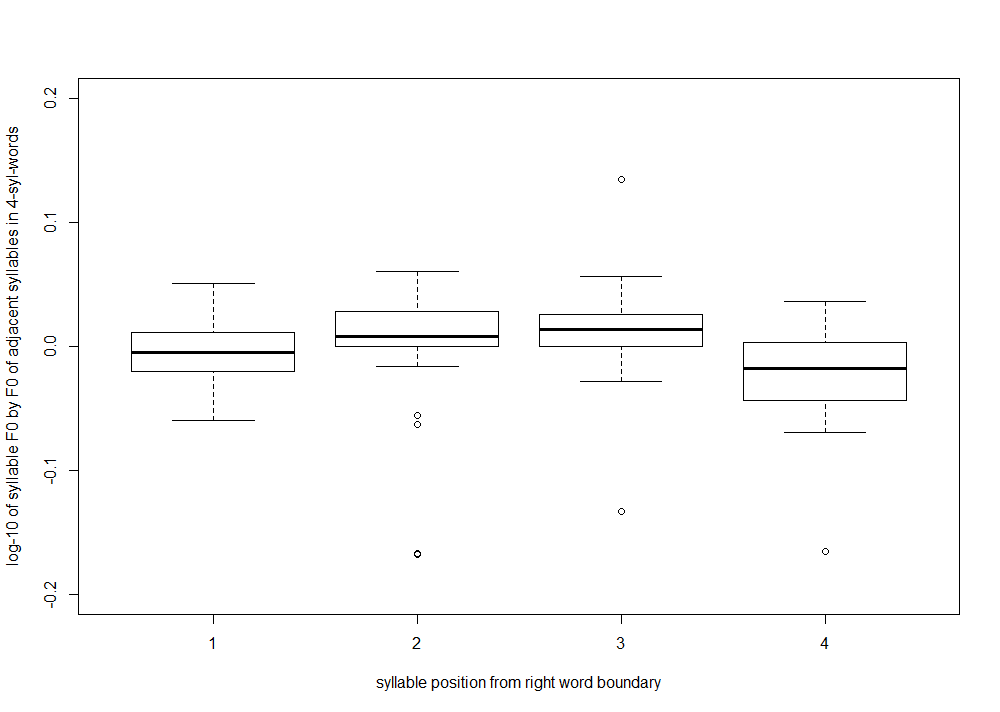
\includegraphics[width=\textwidth]{figures/BUC-img7.png}
%\caption{
%Boxplots of left-right mean F0 coefficient by \isi{syllable position} from the \isi{right word boundary}, only words of \isi{syllable} length 4. \\
%N(1) = 28; 
%N(2) = 44; 
%N(3) = 43; 
%N(4) = 31
%}
%\label{fig:buc:7}
%\end{figure}

This ties in with observations we made inspecting the corpus individually: the main tonal movements seem to be a fall on the penult, often combined with a severe reduction of the last \isi{syllable}, and a less pronounced initial rise. At the phrase level, a similar pattern manifests, of a (phrase-)initial rise, slow downtrend throughout the phrase and additional movement on the penultimate and last \isi{syllable} (see \figref{fig:buc:5}  as a good example of the overall persisting pattern) – note that there is considerable variance on the values of the last two syllables of the phrase, likely due to additional phrase-final movement used to encode assertions and questions, or finalizations and continuations. Comparing the F0 values for the phrase and word levels, there is an indication that a considerable falling movement often takes place over the last three syllables - but this is the case for both words and phrases, so it is hard to tell whether it is indeed a word- or a phrase-level effect.

\begin{figure}
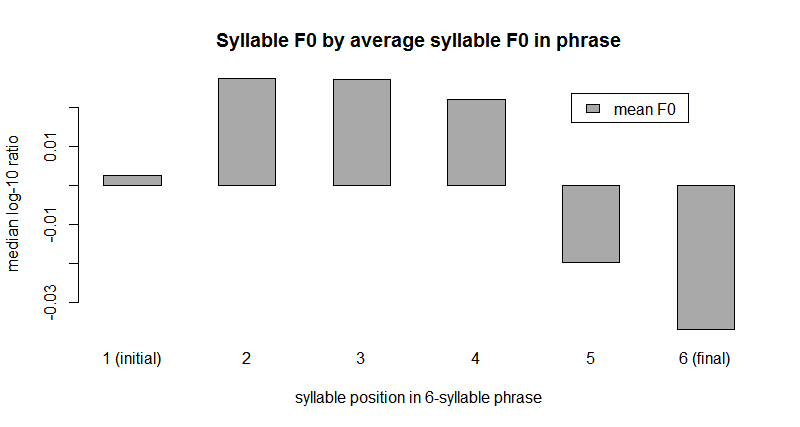
\includegraphics[width=\textwidth]{figures/BUC-img5_new.png}
\caption{Barplots of median log-10 ratios of mean F0 per syllable divided by average mean F0 per syllable in phrases of syllable length 6, ordered according to syllable position in the phrase from left to right. N (1/initial) = 13; N (2) = 15; N (3) = 15; N (4) = 15; N(5) = 15; N (6/final) = 15}
\label{fig:buc:5}
\end{figure}

At least at the phrase-level, the shape of the overall movement can be taken as good evidence for phrasing in the domain of something like an \isi{intonational phrase} – i.e. as evidence that what has here been labeled “phrase” indeed largely captures a phrase in the phonological sense. If the findings of a similar intonational shape across the word or a unit approximating it in size turned out to be robust, this would count as evidence for a lower-level type phrase as well. Whether this lower-level domain corresponds to the word or rather a small phrase above the morphosyntactic word such as an extended NP with preceding adjectives or a PP with embedded Noun, is another question.

\subsubsection{Duration}
Our variety of \ili{Quechua} uses \isi{vowel} length to distinguish meanings both at the level of lexemes and that of grammatical suffixes, for example \textit{wata} `year' vs. \textit{wa\textipa:ta} `domestic animal” vs. \textit{wa\textipa:ta\textipa:} (keep.animals.1s) `I keep it [i.e. an animal]' (cf. \citealt{Parker1976}: 51). As can be seen from these examples and from the literature, the positioning and multiple occurrence of such lengthened syllables is not constrained at the word level. However, when a \isi{syllable} that has a long nucleus and is open is combined with a suffix beginning with two consonants, the first of those becomes the coda of the first \isi{syllable}, and the \isi{vowel} is said to be shortened (CV\textipa: + CCV -> CVC.CV, with the exceptions of nominal roots ending in a long \isi{vowel} and the \isi{vowel} lengthening used to encode verbal first person) in order to conform to a maximal \isi{syllable structure} of CVC or CV\textipa: (cf. \citealt{Parker1976}: 51–52). Nonetheless, as already mentioned, in our data we find a large number of instances of severely reduced word- or phrase-final syllables, which effectively yields spoken “super heavy” final syllables with structures like CVCC or CV\textipa:CC from a combination of the penult with this reduced \isi{final syllable}. Hence it seems that often, the difference between long and short vowels manifests as unreduced but short vs. fully elided vowels. Apart from contravening proposed constraints on the \isi{syllable structure} of our variety of \ili{Quechua}, this process of course also has the effect of shifting \isi{syllable position} from the \isi{right word boundary} one step to the right (the “original” penult with the reduced \isi{final syllable} becoming the “new” \isi{final syllable}). In this situation, our expectation is not to find a straightforward encoding of a fixed prominent position at the word level by means of duration. Indeed, the results of plotting the left-right-coefficient for duration against \isi{syllable position} from the \isi{right word boundary} are very similar to those of the overall coefficient already discussed: basically no large outstanding differences between the positions, especially between penult and ultima (see \figref{fig:buc:2}). This changes again when only considering words of length 4, but more interestingly, \isi{syllable structure} has a much stronger effect: \figref{fig:buc:6} compares the same measurements restricted to syllables of the form CV (orange) to those of the form CVC (purple).\largerpage[-1]   

\begin{figure}
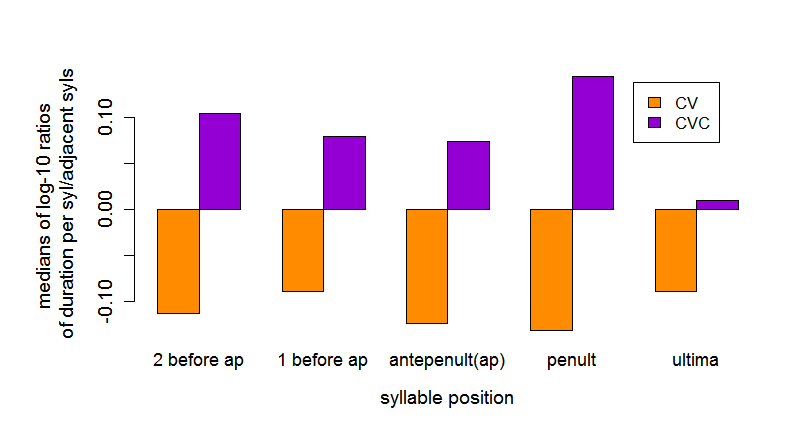
\includegraphics[width=\textwidth]{figures/BUC-img6_new.png}
\caption{Barplots comparing medians of log-10 ratios of the left-right coefficient for duration between CV-syllables (orange) and CVC-syllables (purple), ordered according to syllable position in the word from the right word boundary. For CV-syllables: N (2 before antepenult) = 7; N (1 before antepenult) = 28; N (antepenult) = 67; N (penult) = 126; N (ultima) = 119. For CVC-syllables:  N (2 before antepenult) = 4; N (1 before antepenult) = 7; N (antepenult) = 41; N (penult) = 84; N (ultima) = 79
}
\label{fig:buc:6}
\end{figure}


%\begin{figure}
%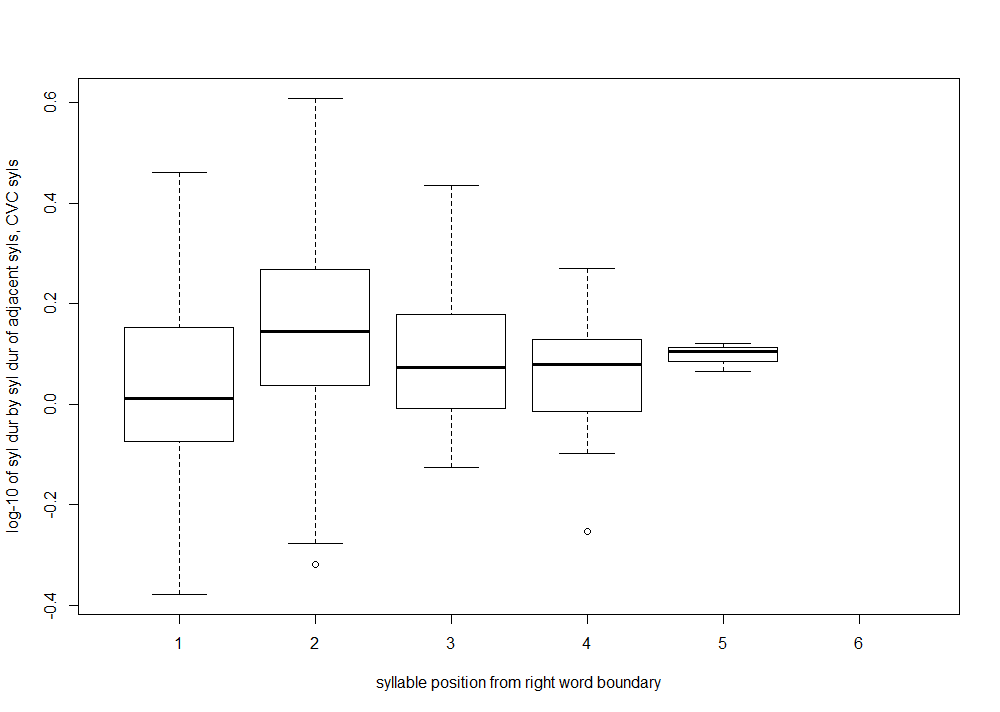
\includegraphics[width=\textwidth]{figures/BUC-img10.png}
%\caption{Boxplots of log-10 of duration of CVC-syllables divided by syllable duration of left- and right-adjacent syllables (y-axis), by position from the right word boundary (x-axis). \\
%N(1) = 79; 
%N(2) = 84; 
%N(3) = 41; 
%N(4) = 7; 
%N(5) = 4
%}
%\label{fig:buc:10}
%\end{figure}


Penults of the form CVC seem to be much longer than their surrounding syllables in comparison with penults of the form CV. Note also that the scale of the y-axis here indicates much larger differences than e.g. in the overall results (\figref{fig:buc:2}). Consider here that we cannot tell whether the adjacent syllables for each individual \isi{syllable} of this form also had the same form, thus it is possible that all of the penultimate CVC syllables were surrounded by syllables of shorter structure. If that were the case however, it would suggest a distribution of CVC-syllables sensitive to \isi{syllable position} within the word, which would contradict Parker’s description and would be interesting in itself. However, it would also be the case that a large share of the syllables in word-final position annotated here as CVC are the product of \isi{final syllable} reduction and are thus “former” penults. Thus, if a process existed to produce penults of the form CVC, it would work against that one producing final syllables of that form. In fact, many of the CVC-penults might actually have ended up as final syllables in this data, but the relative length distinction persists. It is thus plausible that syllables in penultimate position receive some kind of \isi{prominence} that is realized at least partially through duration, but that this is often obscured by the length difference realized on behalf of \isi{syllable structure}. As with all findings presented here, this one also needs to be supported by further analysis of a larger dataset.   

\largerpage
\subsubsection{Intensity} 
Intensity is usually not a very good correlate of metrical \isi{prominence} in most languages, although it was once thought to be the main correlate in languages with word-level stress \citep{Beckman1986}. Here, it presents an interesting addition to the results so far: From \figref{fig:buc:2}, we can see that of all measures of \isi{realizational strength} we have looked at so far, intensity (green) shows the penult to stand out from the other positions most clearly without the application of any further conditions. However, looking at the scale for the y-axis in Figure 2, we can see that none of the parameters there reach a median value above 0.04 (corresponding to a ratio of 1.096478 to 1), so also the strength of the effect of intensity here should not be overestimated.

%\begin{figure}
%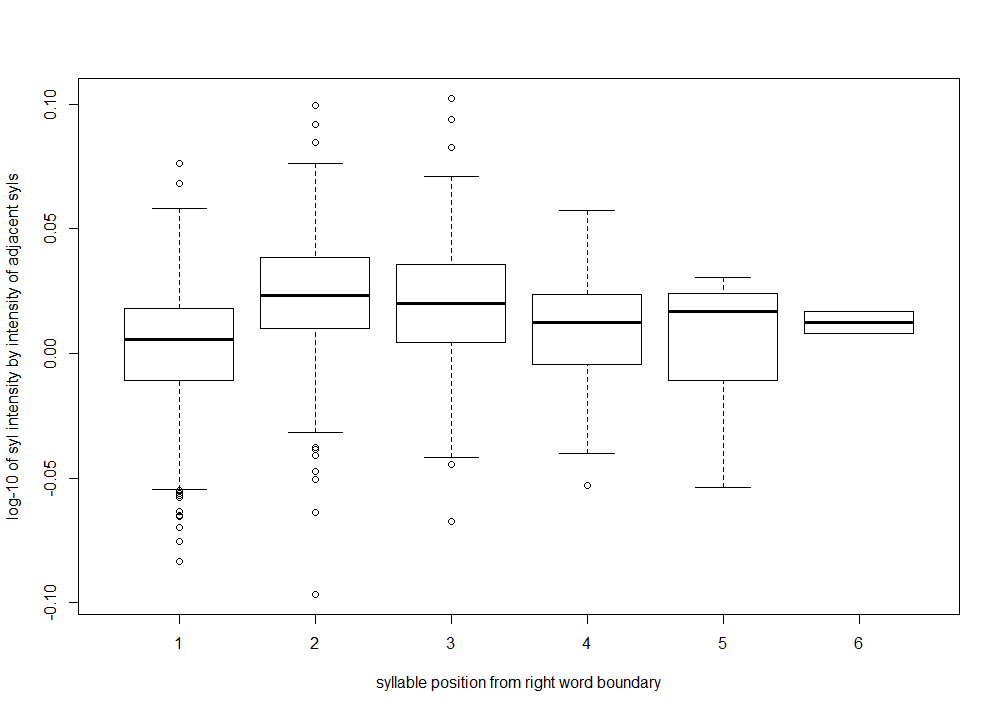
\includegraphics[width=\textwidth]{figures/BUC-img11.png}
%\caption{Boxplots of left-right intensity coefficient by syllable position from the right word boundary, entire sample. \\
%N(1) = 255; 
%N(2) = 281; 
%N(3) = 136; 
%N(4) = 49; 
%N(5) = 11; 
%N(6) = 2
%}
%\label{fig:buc:11}
%\end{figure}

\subsection{Information structural categories}
In many proposals, information structural categories play an important role for the assignment of \isi{prominence} at a high level of \isi{prosodic} structure. Especially, the category of focus is often associated with a particular \isi{pitch accent} (\citealt{Buering2012}, among many others) and many language specific annotation systems (ToBIs) implementing the autosegmental-metrical model of \isi{intonation} \citep{Pierrehumbert1980} include different intonational categories for different kinds of foci such as information focus and \is{focus!contrastive}contrastive focus, including the ToBI for peninsular \ili{Spanish} Sp\_ToBI (\citealt{Beckman.2002}; \citealt{EstebasVilaplanaPrieto.2008}). An additional assumption that has been proven empirically for many languages is that such high-level \isi{prominence} markings of foci occur at the same site as other word- or phrase-level prominences, i.e. that a focused word will receive a particular accentual \isi{prominence} on the \isi{syllable} that is metrically already most prominent. Several recent proposals have cast the universality of this claim into doubt (cf. \citealt{Kuegler2012,Fery2013}). It seems to be the case that at least in some languages, the hierarchy of focus strength proposed in \citet[688--690]{Fery2013}, going from broad information focus to narrow corrective focus necessitates a realization via marked \isi{prosody} only at higher points of the scale. It is nevertheless promising to look for loci of \isi{prominence} via information structural categories. It comes as somewhat of a surprise, then, that no clear overall results are obtained when applying this difference in labeling. Reasons for this might lie in the relatively broad labeling decision regarding focus (see \sectref{sec:buc:3.3.2}), which might have to be refined for further studies, adopting Féry’s hierarchy of focus strength, and which could allow for too much variation, or in the sample size. The same holds for the difference between those syllables labelled as “given”, and those labelled as “new”, and again speculation about reasons for this will lead us most immediately to categories labelled too broadly and the small sample size. However, a distinction that does yield interesting results is the one between topic and comment. See \figref{fig:buc:7} for a comparison of the values for topic (dark green) and comment (blue). Why this is the one information structural category yielding mentionable results (again favoring the penultima), is at this stage open to speculation. A possible factor might be that topics that are fully realized are often \is{topic!contrastive}contrastive topics or topic shifts and hence focal in the sense that they evoke salient alternatives; the way the data was annotated has a bias towards labeling parts of utterances of comment insofar as that utterances without realized topics were labelled as “comment”  (and not e.g. as “thetic”), so “topic” might actually often label a subset of focused parts of speech, namely those  focused contrastively. Contrastive foci rank relatively high in Féry’s hierarchy of focus strength and are thus more likely to be realized with marked \isi{prosody} in her account.   

\begin{figure}
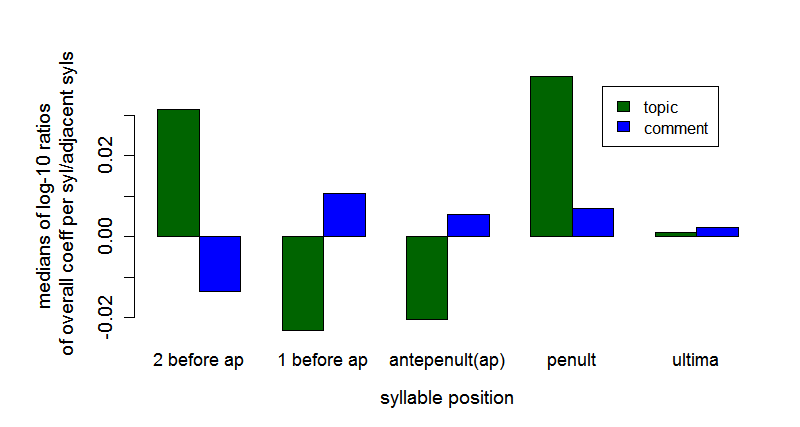
\includegraphics[width=\textwidth]{figures/BUC-img7_new.png}
\caption{Barplots comparing medians of log-10 ratios of the overall left-right coefficient between syllables labeled “topic" (dark green) and “comment" (blue), ordered according to syllable position in the word from the right word boundary. For “topic": N (2 before antepenult) = 5; N (1 before antepenult) = 15; N (antepenult) = 37; N (penult) = 93; N (ultima) = 84. For “comment": N (2 before antepenult) = 6; N (1 before antepenult) = 33; N (antepenult) = 97; N (penult) = 180; N (ultima) = 194
}
\label{fig:buc:7}
\end{figure}

%\begin{figure}
%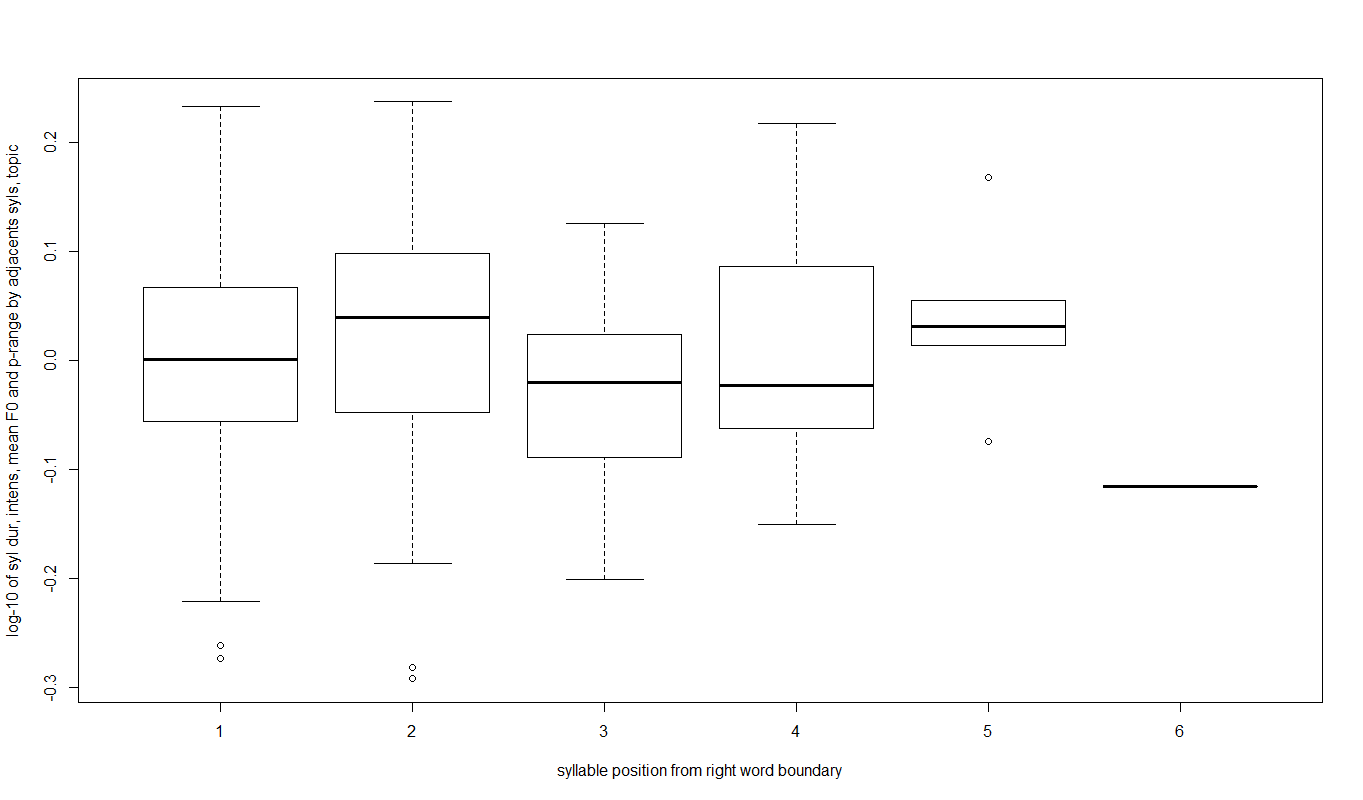
\includegraphics[width=\textwidth]{figures/BUC-img12.png}
%\caption{Boxplots of left-right overall coefficient by syllable position from the right word boundary, only syllables labelled “topic”. \\
%N(1) = 84; 
%N(2) = 93; 
%N(3) = 37; 
%N(4) = 15;
%N(5) = 5; 
%N(6) = 1
%}
%\label{fig:buc:12}
%\end{figure}


%\begin{figure}
%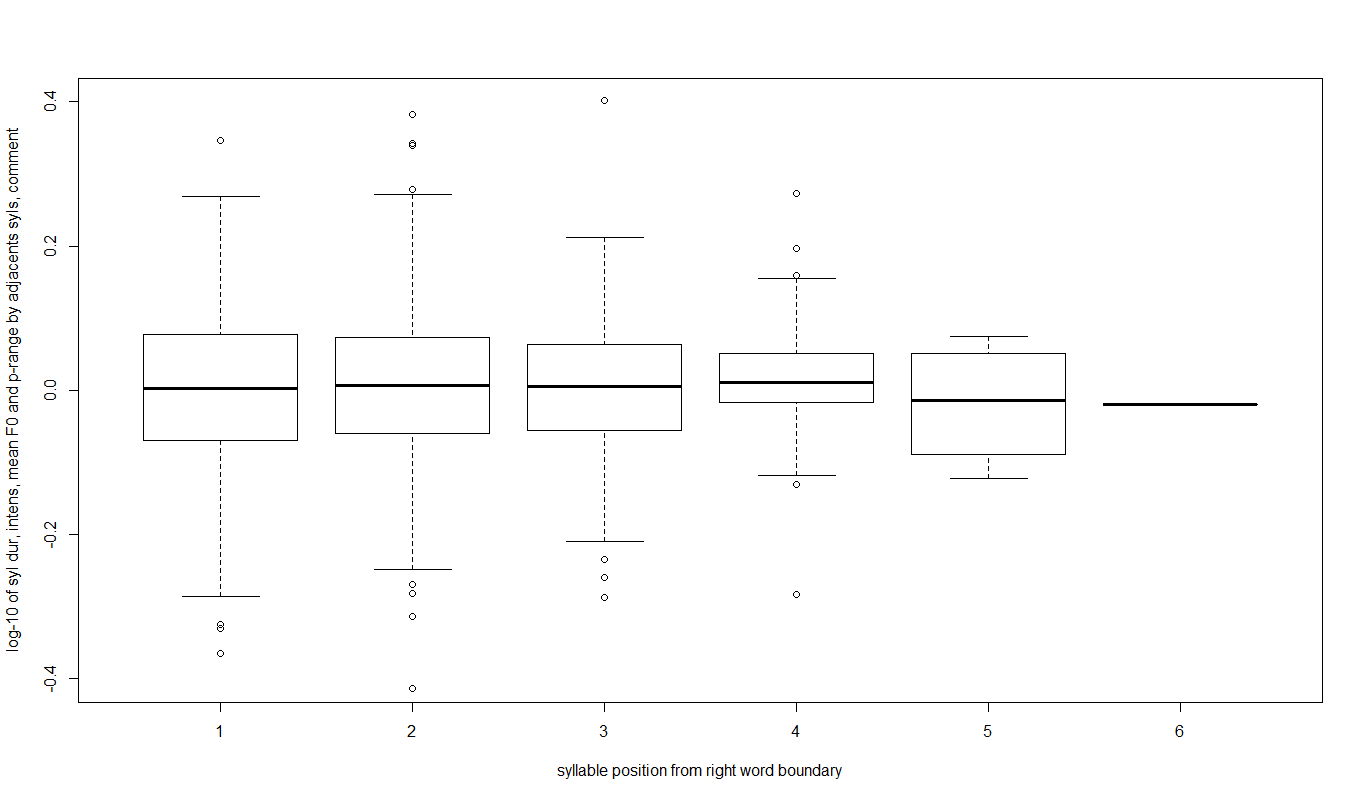
\includegraphics[width=\textwidth]{figures/BUC-img13.png}
%\caption{Boxplots of left-right overall coefficient by syllable position from the right word boundary, only syllables labelled “comment”. \\
%N(1) = 149;
%N(2) = 180; 
%N(3) = 97; 
%N(4) = 33; 
%N(5) = 6;
%N(6) = 1
%}
%\label{fig:buc:13}
%\end{figure}


A related explanation might be that realized topics are often only nominal constituents, again making them a more “narrow” label. Both these explanations receive incidental support by the fact that there is a total of 466 syllables labelled “comment” in the sample used versus only 235 labelled “topic”. Further investigation into this is again needed.
\\

\section{Discussion – what we’ve got, what needs to be done and what’s feasible}
The results we have obtained so far are promising in that they demonstrate that it is indeed possible with this method to say something about consistent positions of \isi{realizational strength} in a language where phonological \isi{prominence} patterns are unknown, thus providing an empirical basis for hypotheses about these positions and the processes affecting their realization. The most convincing result for the utterances analyzed in this pilot corpus is that of \isi{prominence} on the penult of the (\isi{prosodic}) word, as demonstrated by the overall coefficient for 4-\isi{syllable} words and under the condition topic and \isi{pitch range}; duration when controlled for \isi{syllable structure} and intensity overall. A second result is that of a possible secondary \isi{prominence} on the \isi{initial syllable}, as indicated by the overall and \isi{pitch range} coefficient on 4-\isi{syllable} words, and that for duration of CVC syllables. The most general caution regarding any of these hypotheses concerns the size and lack of balance of the corpus, and the consequent lack of any inferential statistics corroborating the general applicability of the results’ predictions. We intend to improve upon this state of affairs with a follow-up study on a larger sample. More specific limitations are discussed in the following. It would be useful to test the method as explained here on a comparable corpus of a language where \isi{prominence} positions are well known, such as peninsular \ili{Spanish}.\footnote{We thank Paolo Roseano for this and several other very useful suggestions on how to improve this work.}  This is also something we intend to remedy in the future. Comparable research, reported on in Pamies Bertrán (\citeyear{PamiesBertran1994} and especially \citeyear{PamiesBertran1996}), has also used a coefficient composed of ratios of one acoustic parameter for one \isi{syllable} by that of its neighbors to study acoustic realization of prominent positions in several languages where these positions are known. Although the calculations used to derive at his results, described in \citet[27--29]{PamiesBertran1996}, remain somewhat vague, the results themselves are similarly promising in that they suggest a general realization of prominences by a combination of these cues and a compensatory mechanism between them that is at work to differing degrees in the different languages under his discussion. His sample size for each of the seven languages analyzed (\ili{Catalan}, English, \ili{French}, \ili{Italian}, \ili{Portuguese} (lumping European and \ili{Brazilian Portuguese} together, which we find questionable from a \isi{prosodic} point of view), Russian and \ili{Spanish}) is even smaller than ours for \ili{Quechua}, hence the same general limitations apply. However, one very consistent result of his (reported on at greater length for \ili{Spanish} in \citealt{PamiesBertran1994}) is that prominent positions adjacent to each other (“acentos contiguous” in his terminology, “stress clash” more generally) do not allow for a consistently strong realization by any of the parameters. This has a possible bearing on our results as well, since it might help explain why no good results could be obtained in almost any condition for 2- and 3-\isi{syllable} words. This would follow immediately if both the penult and the \isi{initial syllable} were indeed prominent, creating clashes to be resolved by the \isi{phonetic} realization (see also \citealt{Hintz2006} for a similar observation on a central \ili{Quechua} variety very close to ours). It would especially be the case if what is seen as realizationally strong in the initial is mainly a rise in F0, whereas being a combination of a fall in F0 plus intensity and optional durational \isi{prominence} in the penult; the rises and falls would conflict in 2-\isi{syllable} words and create movements that cannot be disentangled by this method alone. This is one of the more specific limitations of this method, i.e. that in the domain of \isi{intonation} it cannot properly differentiate between such phenomena as late and early peaks. The comparison of the coefficients for mean F0 and \isi{pitch range} does allow for some more fine-grained intonational profiling of words of a given length, but it cannot resolve the issue of consistently late peaks versus peaks within the accented \isi{syllable} by itself. Another related issue is that of reduction and \isi{prosodic phrasing}. While in theory it would be possible to calculate mean constellations of F1--F2 for each intended \isi{vowel} type in the corpus and then calculate their reduction by centralization by measurement of Euclidean distances from that mean and their durational reduction for each individual \isi{vowel} token, in practice this would mean individually checking each \isi{vowel} due to issues in automatic formant measurement in {Praat}, greatly reducing the advantage of automatization this method aims at. Hence, the clearly existing reduction processes in our variety of \ili{Quechua} are not very well captured by this method. However, they are prime candidates as indicators for \isi{prosodic} boundaries and hence very important to our general endeavor of determining \isi{prominence} positions. To sum up and refine our desires for further investigations, they should therefore consist of acoustic measurements of the kind described here on a larger corpus of utterances where reductions are annotated as \isi{prosodic} boundaries, preferably on ones of \isi{syllable} length 4 and greater in order to better disentangle primary and secondary prominences and their differing realizations.    

\section*{Acknowledgments}
The research presented here has been conducted as part of the DFG-funded project \textit{Zwei\-sprachige Prosodie: Rhythmus, Metrik und Intonation zwischen Spanisch und Quechua} at FU Berlin. As part of this project, we undertook a fieldtrip to Huari, Conchucos, Peru in the summer of 2015, from which the data used in this research stems. We very gratefully acknowledge the support of the Deutsche Forschungsgemeinschaft and would also like to thank the speakers we recorded for their time and willingness to participate in our experiments.

{\sloppy
\printbibliography[heading=subbibliography,notkeyword=this]
}



\end{document}
